\chapter{\ifproject%
\ifenglish Project Structure and Methodology\else โครงสร้างและขั้นตอนการทำงาน\fi
\else%
\ifenglish Project Structure\else โครงสร้างของโครงงาน\fi
\fi
}

% ในบทนี้จะกล่าวถึงหลักการ และการออกแบบระบบ

\makeatletter

% \renewcommand\section{\@startsection {section}{1}{\z@}%
%                                    {13.5ex \@plus -1ex \@minus -.2ex}%
%                                    {2.3ex \@plus.2ex}%
%                                    {\normalfont\large\bfseries}}

\makeatother
%\vspace{2ex}
% \titleformat{\section}{\normalfont\bfseries}{\thesection}{1em}{}
% \titlespacing*{\section}{0pt}{10ex}{0pt}



\section{หลักการทำงานของแอปพลิเคชัน}
โครงงานนี้เป็นแอปพลิเคชันที่ช่วยในการสร้าง, ประกาศกิจกรรม และเข้าร่วมกิจกรรมของนักศึกษาของมหาวิทยาลัยเชียงใหม่
โดยเลือกพัฒนาเป็นเว็บแอปพลิเคชัน มีระบบที่ให้ผู้ใช้สร้างและประชาสัมพันธ์กิจกรรม, ดูข้อมูลและขอเข้าร่วมกิจกรรมที่ตนเองสนใจ โดยทางเว็บจะมีระบบแนะนำกิจกรรมที่ตรงกับความสนใจของผู้ใช้มากที่สุด 
\begin{figure}[h] %h = here. other are top,bottom,separate page(p)
\begin{center}
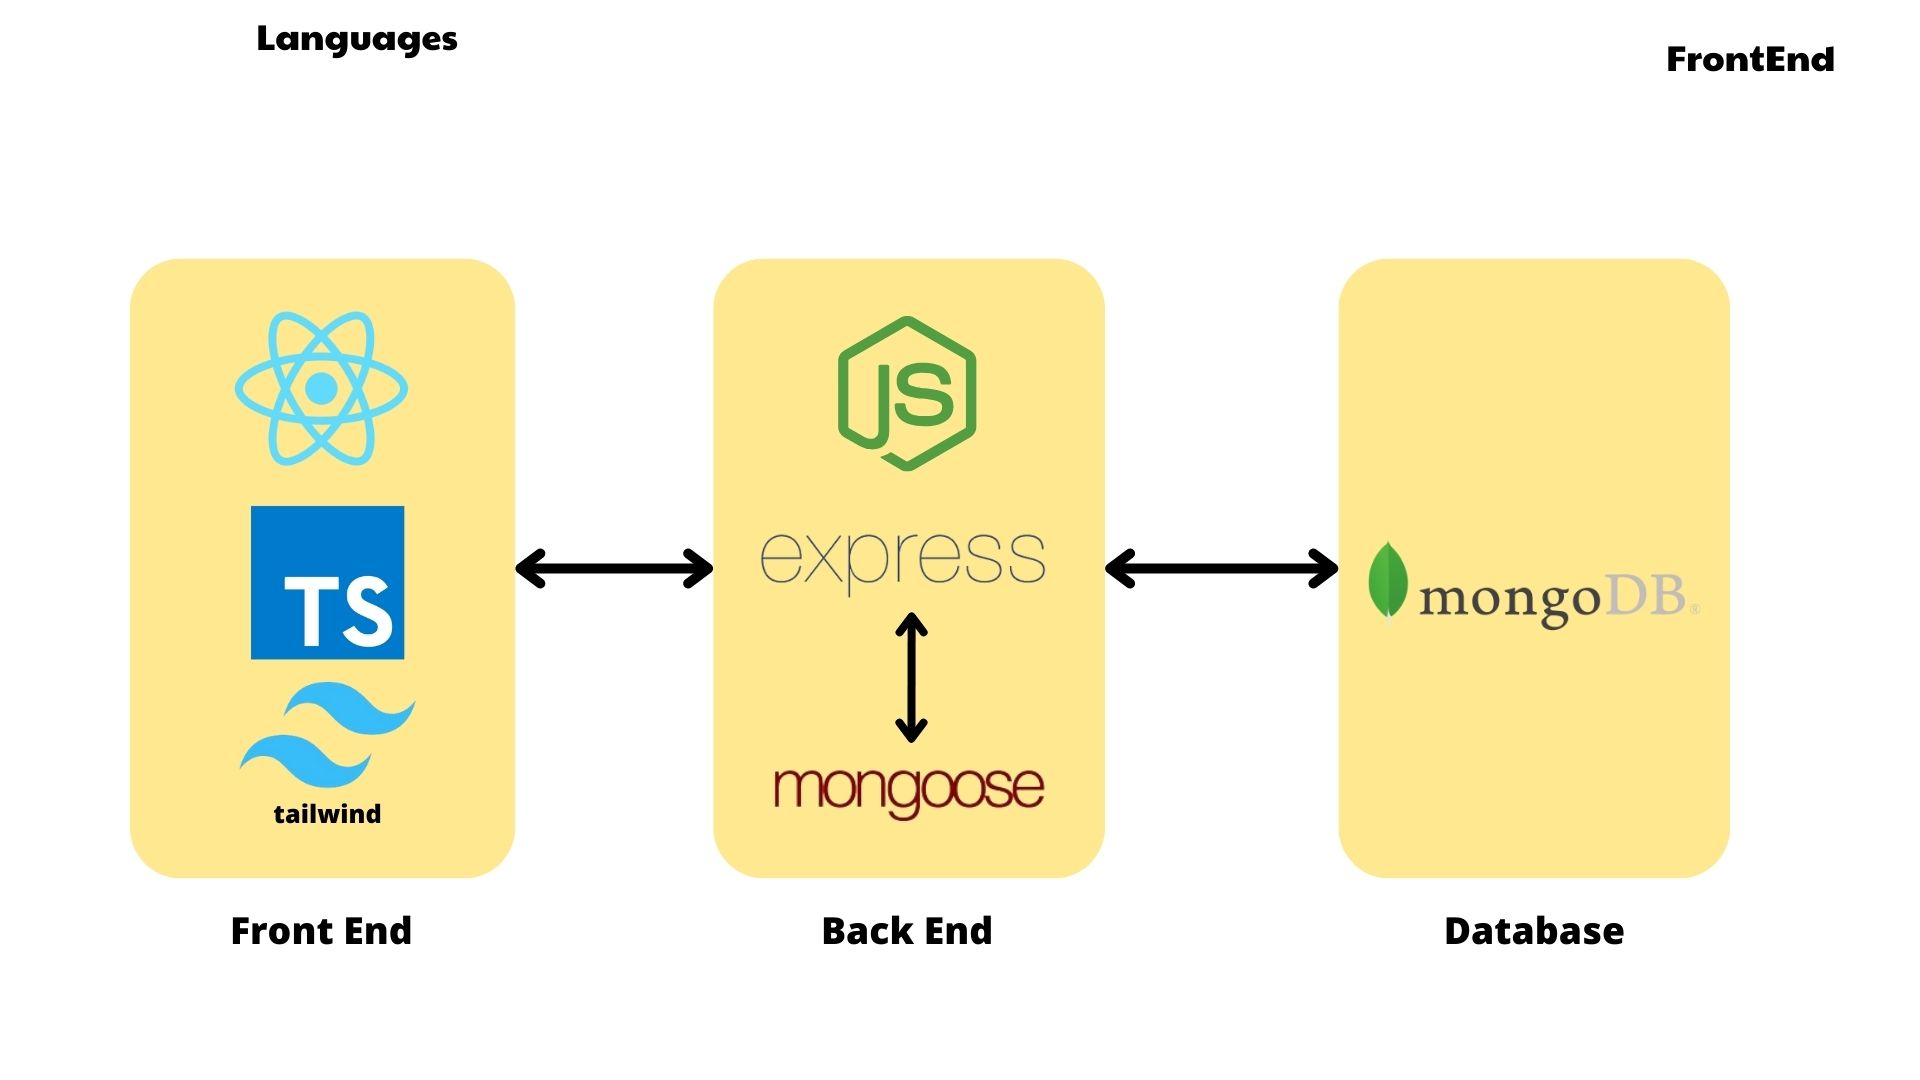
\includegraphics[width=0.9\linewidth]{image/techFlow.jpg}
\end{center}
\caption[หลักการทำงานของแอปพลิเคชัน]{System Overview}
\label{fig:system_overview}
\end{figure}
\section{การใช้งานแอปพลิเคชัน}
เว็บแอปพลิเคชันนี้จะแบ่งกลุ่มผู้ใช้ออกเป็น 2 กลุ่ม ได้แก่
\subsection{ผู้ใช้ทั่วไปที่ยังไม่ได้ลงทะเบียนเข้าสู่ระบบ}
สิ่งที่ผู้ใช้ทั่วไปสามารถใช้งานได้ ได้แก่
\begin{itemize}
    \item สามารถอ่านข่าวรายละเอียดของเว็บไซด์ได้ในหน้าหลัก
    \item สามารถค้นหากิจกรรมที่อยู่ในหน้าข่าวสารกิจกรรมได้
    \item สามารถดูรายละเอียดของแต่ละกิจกรรมได้
\end{itemize}

\newpage

\subsection{ผู้ใช้ที่ลงทะเบียนเข้าสู่ระบบแล้ว}
หลังจากผู้ใช้ลงทะเบียนเข้าใช้งานด้วย email แล้ว สิ่งที่ผู้ใช้สามารถทำได้เพิ่มมากขึ้น ได้แก่
\begin{itemize}
    \item สามารถเปลี่ยนรูปโปรไฟล์ได้
    \item สามารถสร้างกิจกรรมใหม่ได้
    \item กดสนใจกิจกรรมได้
    \item สามารถสมัครเข้าร่วมตำแหน่งที่เปิดรับสมัครได้
    \item สามารถตอบรับคำขอเข้าร่วมกิจกรรมได้หากมีคนขอสมัครกิจกรรมที่ผู้ใข้เป็นผู้สร้าง
    \item สามารถเข้าดูหน้ากิจกรรมของฉันเพื่อดูกิจกรรมที่กดสนใจเข้าร่วมไปแล้วได้
\end{itemize}
\section{นโยบายความเป็นส่วนตัว}
ข้อมูลส่วนตัวของผู้ใช้จะถูกเก็บเป็นความลับจากผู้ใช้คนอื่น โดยจะเปิดเผยแค่ ชื่อ,นามสกุล,ชั้นปี ให้กับผู้สร้างกิจกรรมที่ผู้ใช้กดสมัครไป
\section{การออกแบบหน้าเว็บแอปพลิเคชัน}
ในการออกแบบหน้าเว็บแอปพลิชัน พวกเราได้เลือกใช้ Figma เพราะเป็นเครื่องมือที่อำนวยความสะดวก ในการออกแบบหน้าเว็บแอปพลิเคชัน ช่วยให้การออกแบบ UI/UX สะดวกมากขึ้น อีกทั้งยังเป็นเครื่องมือที่ผู้คนต่างก็นิยมใช้
ทำให้ผู้ใช้ทั่วโลกสามารถแชร์วิธีการออกแบบ ทำให้สามารถนำไปเป็นไอเดียในการออกแบบได้ 
\begin{figure}[h]
  \centering
  \begin{subfigure}[b]{0.4\linewidth}
    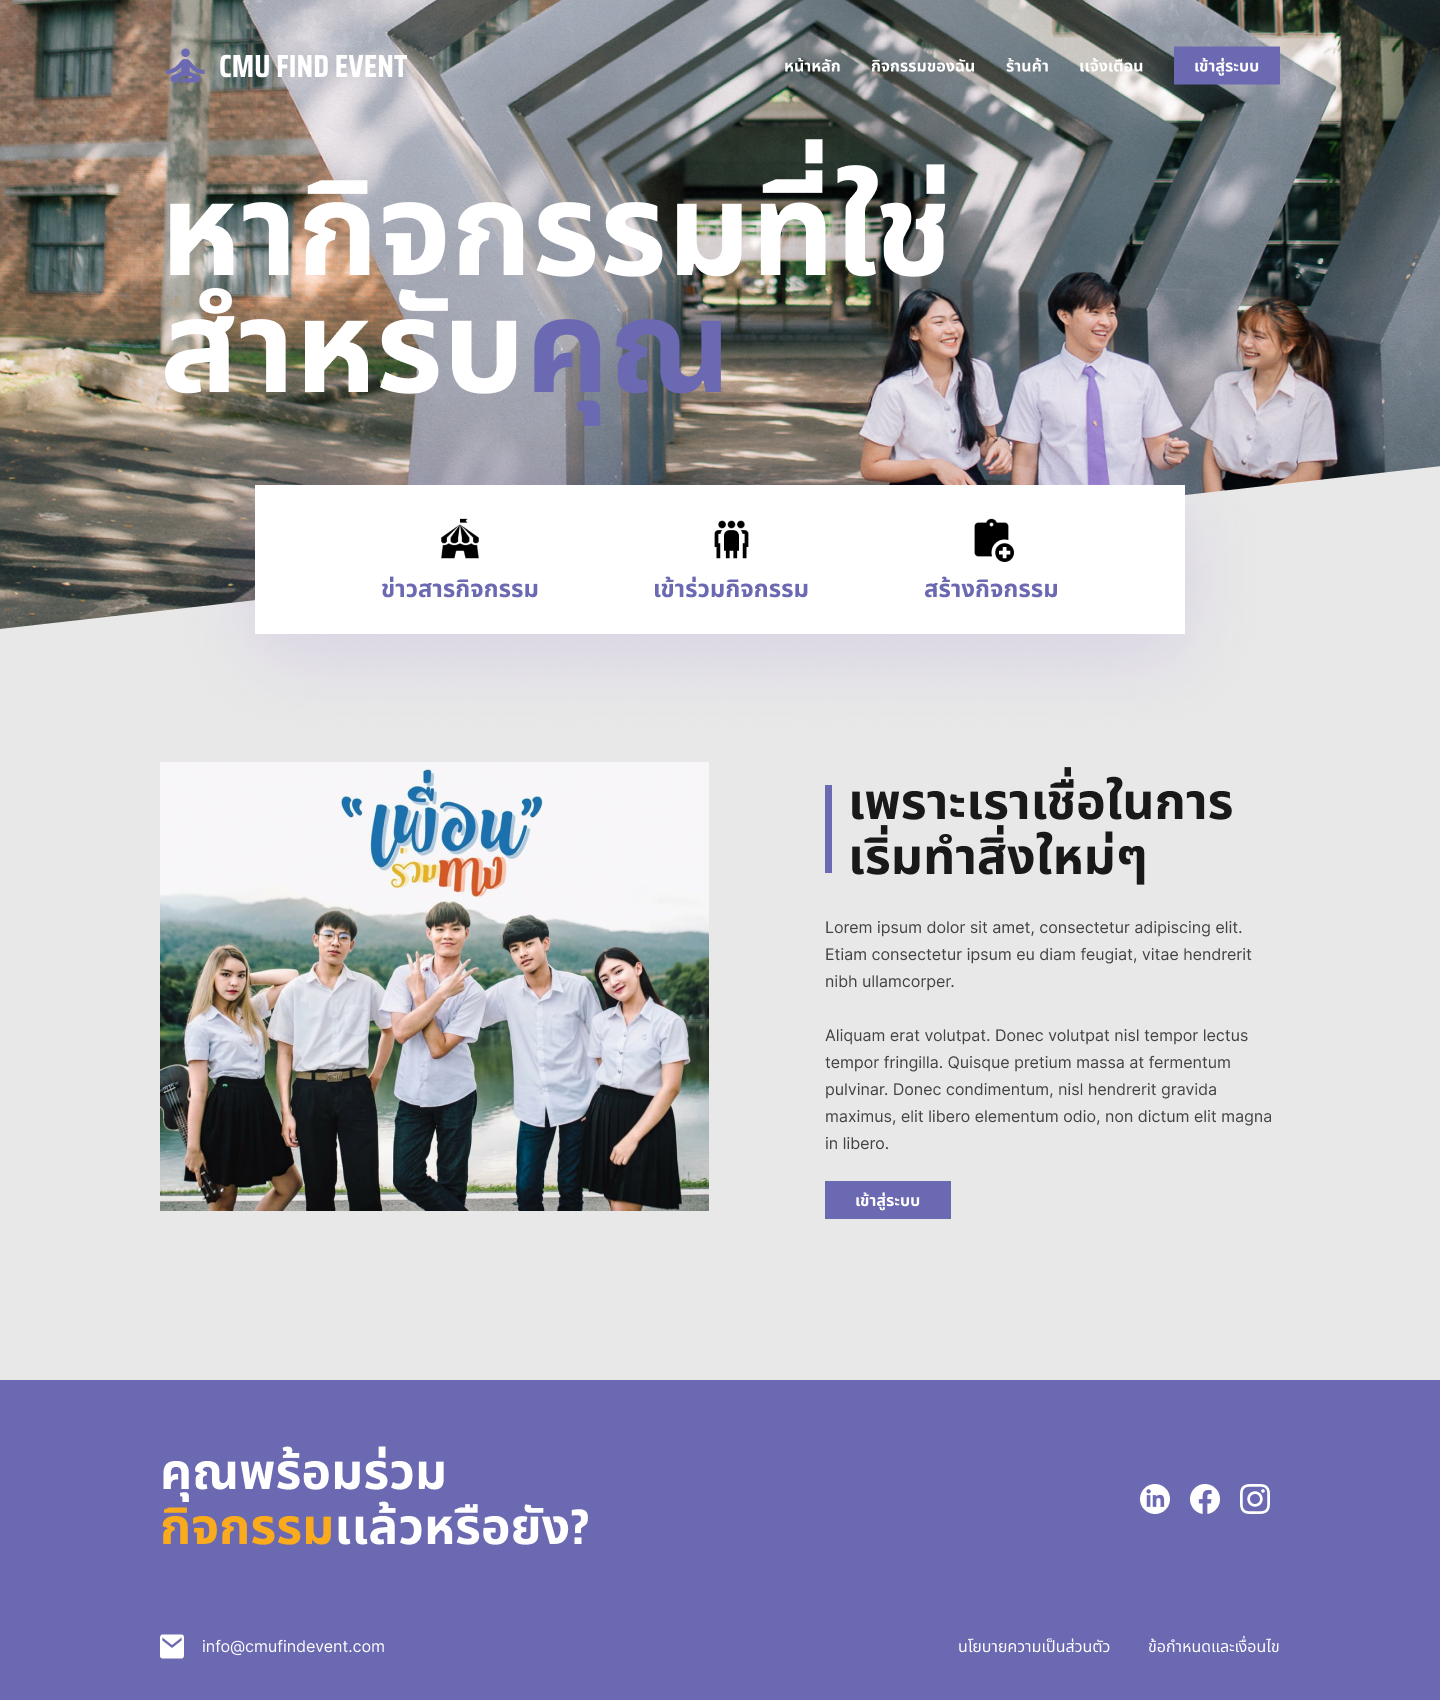
\includegraphics[width=\linewidth]{image/Figma-design/Main-not-login.png}
    \caption{แสดงข้อมูลของเว็บ}
  \end{subfigure}
  \hfill
  \begin{subfigure}[b]{0.4\linewidth}
    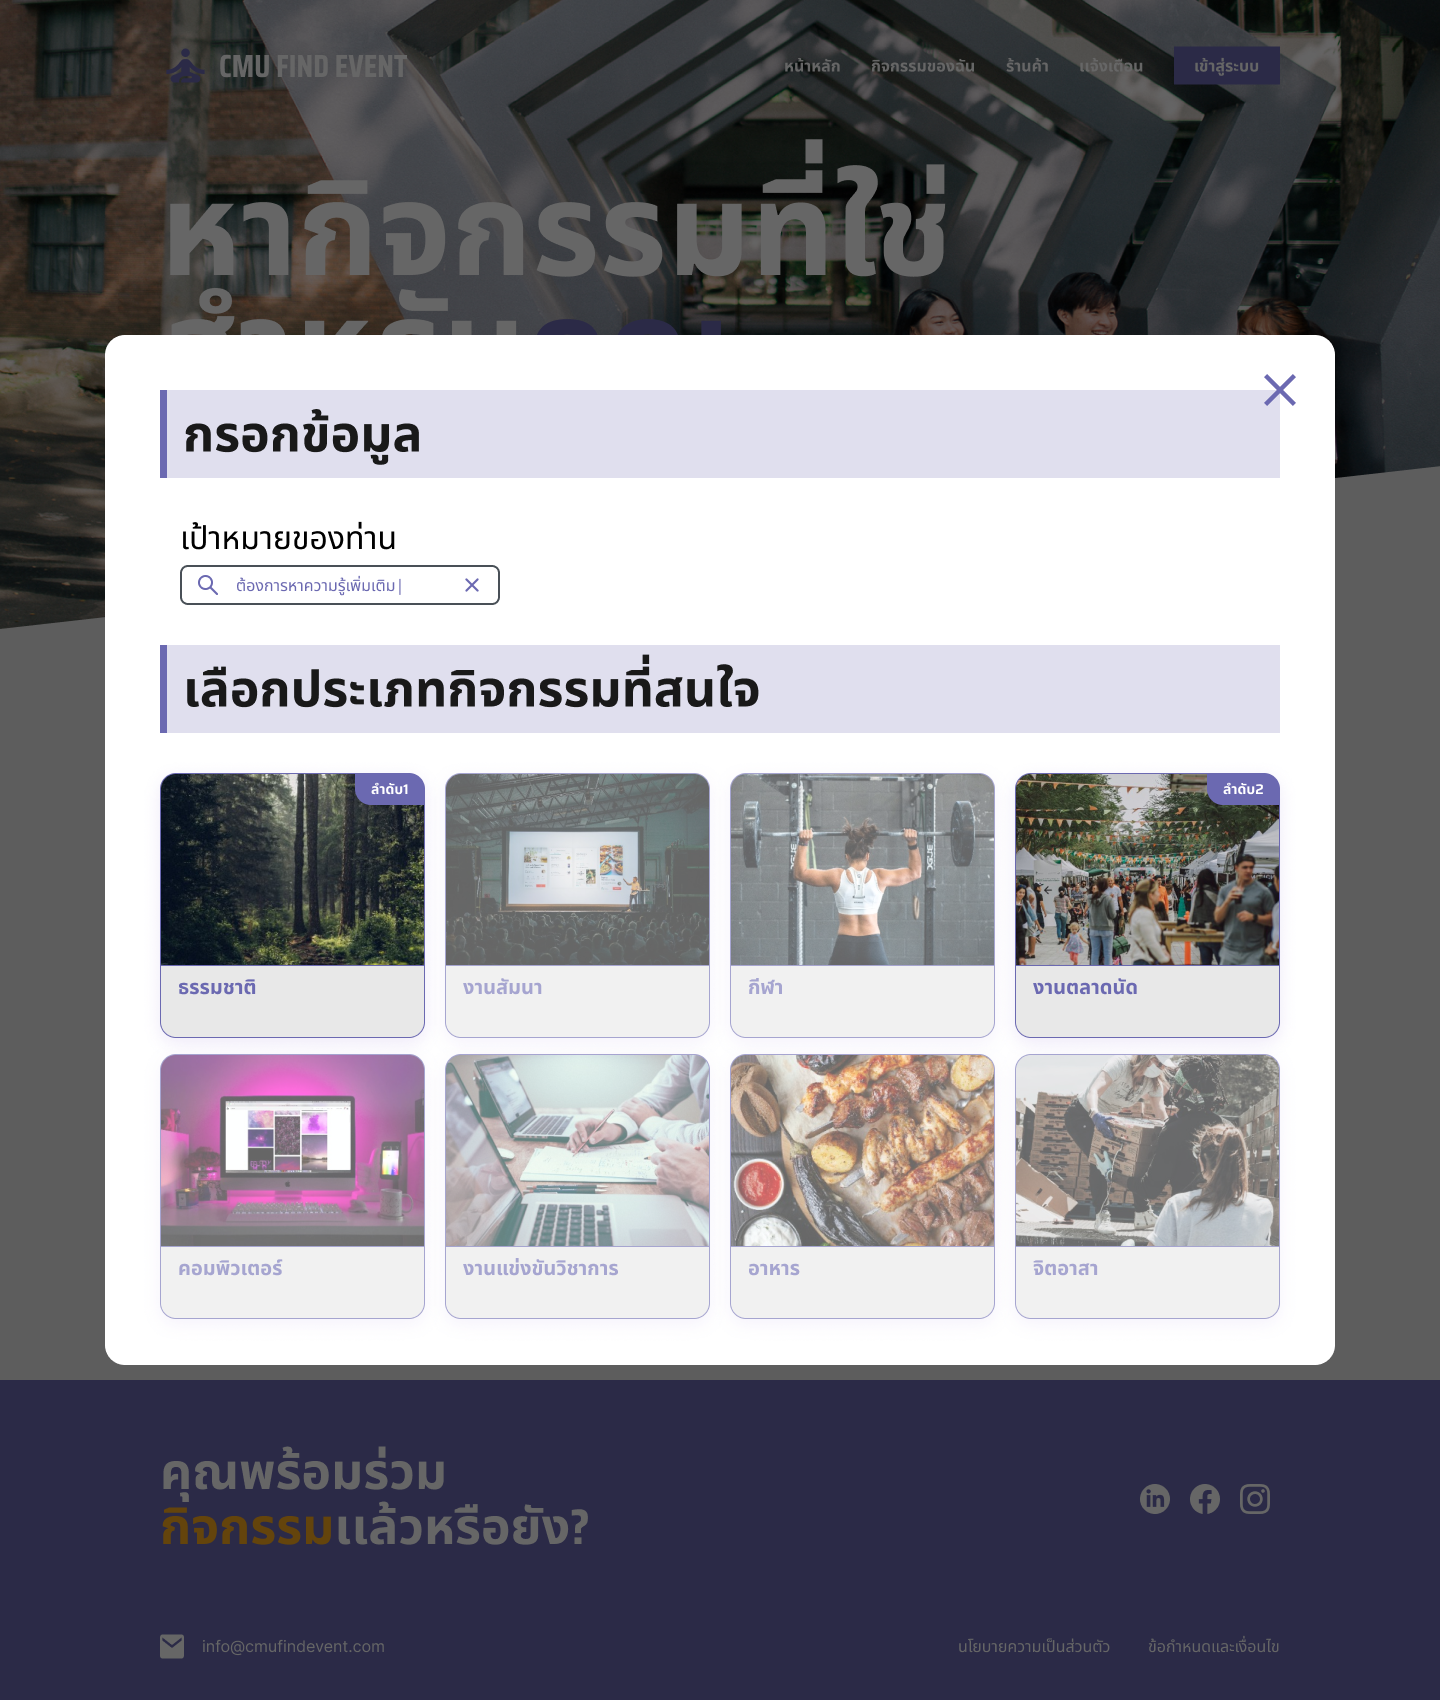
\includegraphics[width=\linewidth]{image/Figma-design/Main-recomendation.png}
    \caption{แสดงแบบสอบถามกิจกรรมที่สนใจ}
  \end{subfigure}
  \caption{หน้าแรก}
  \label{fig:main}
\end{figure}

\begin{figure}[h]
  \centering
  \begin{subfigure}[b]{0.3\linewidth}
    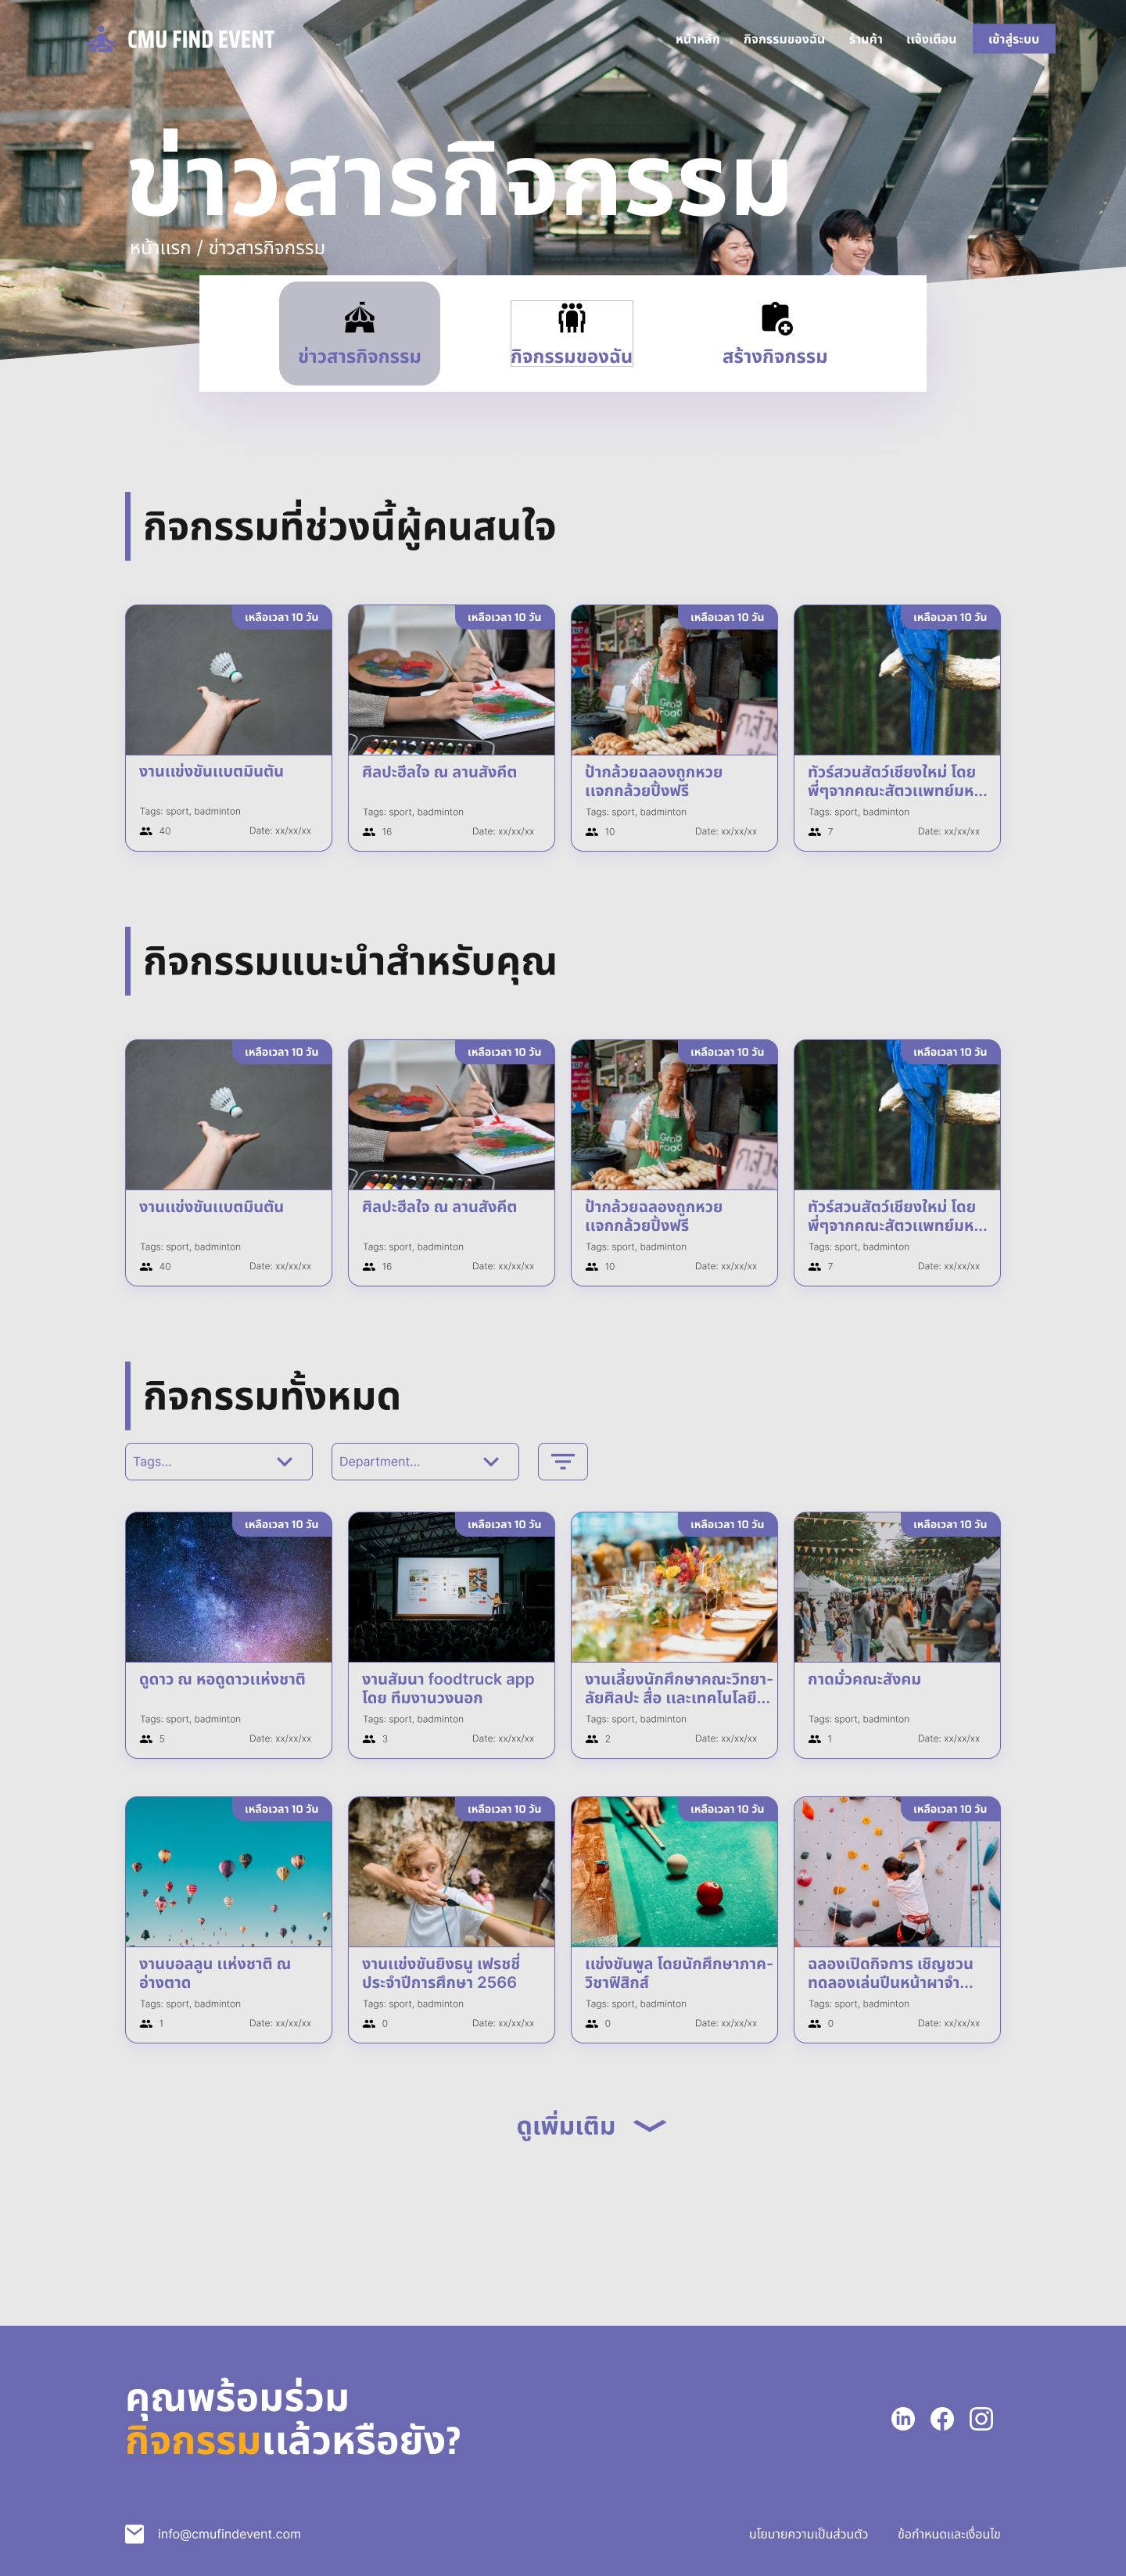
\includegraphics[width=\linewidth]{image/Figma-design/New-Event-info.jpg}
    \caption{แสดงรายการกิจกรรมต่างๆ}
  \end{subfigure}
  \hfill
  \begin{subfigure}[b]{0.3\linewidth}
    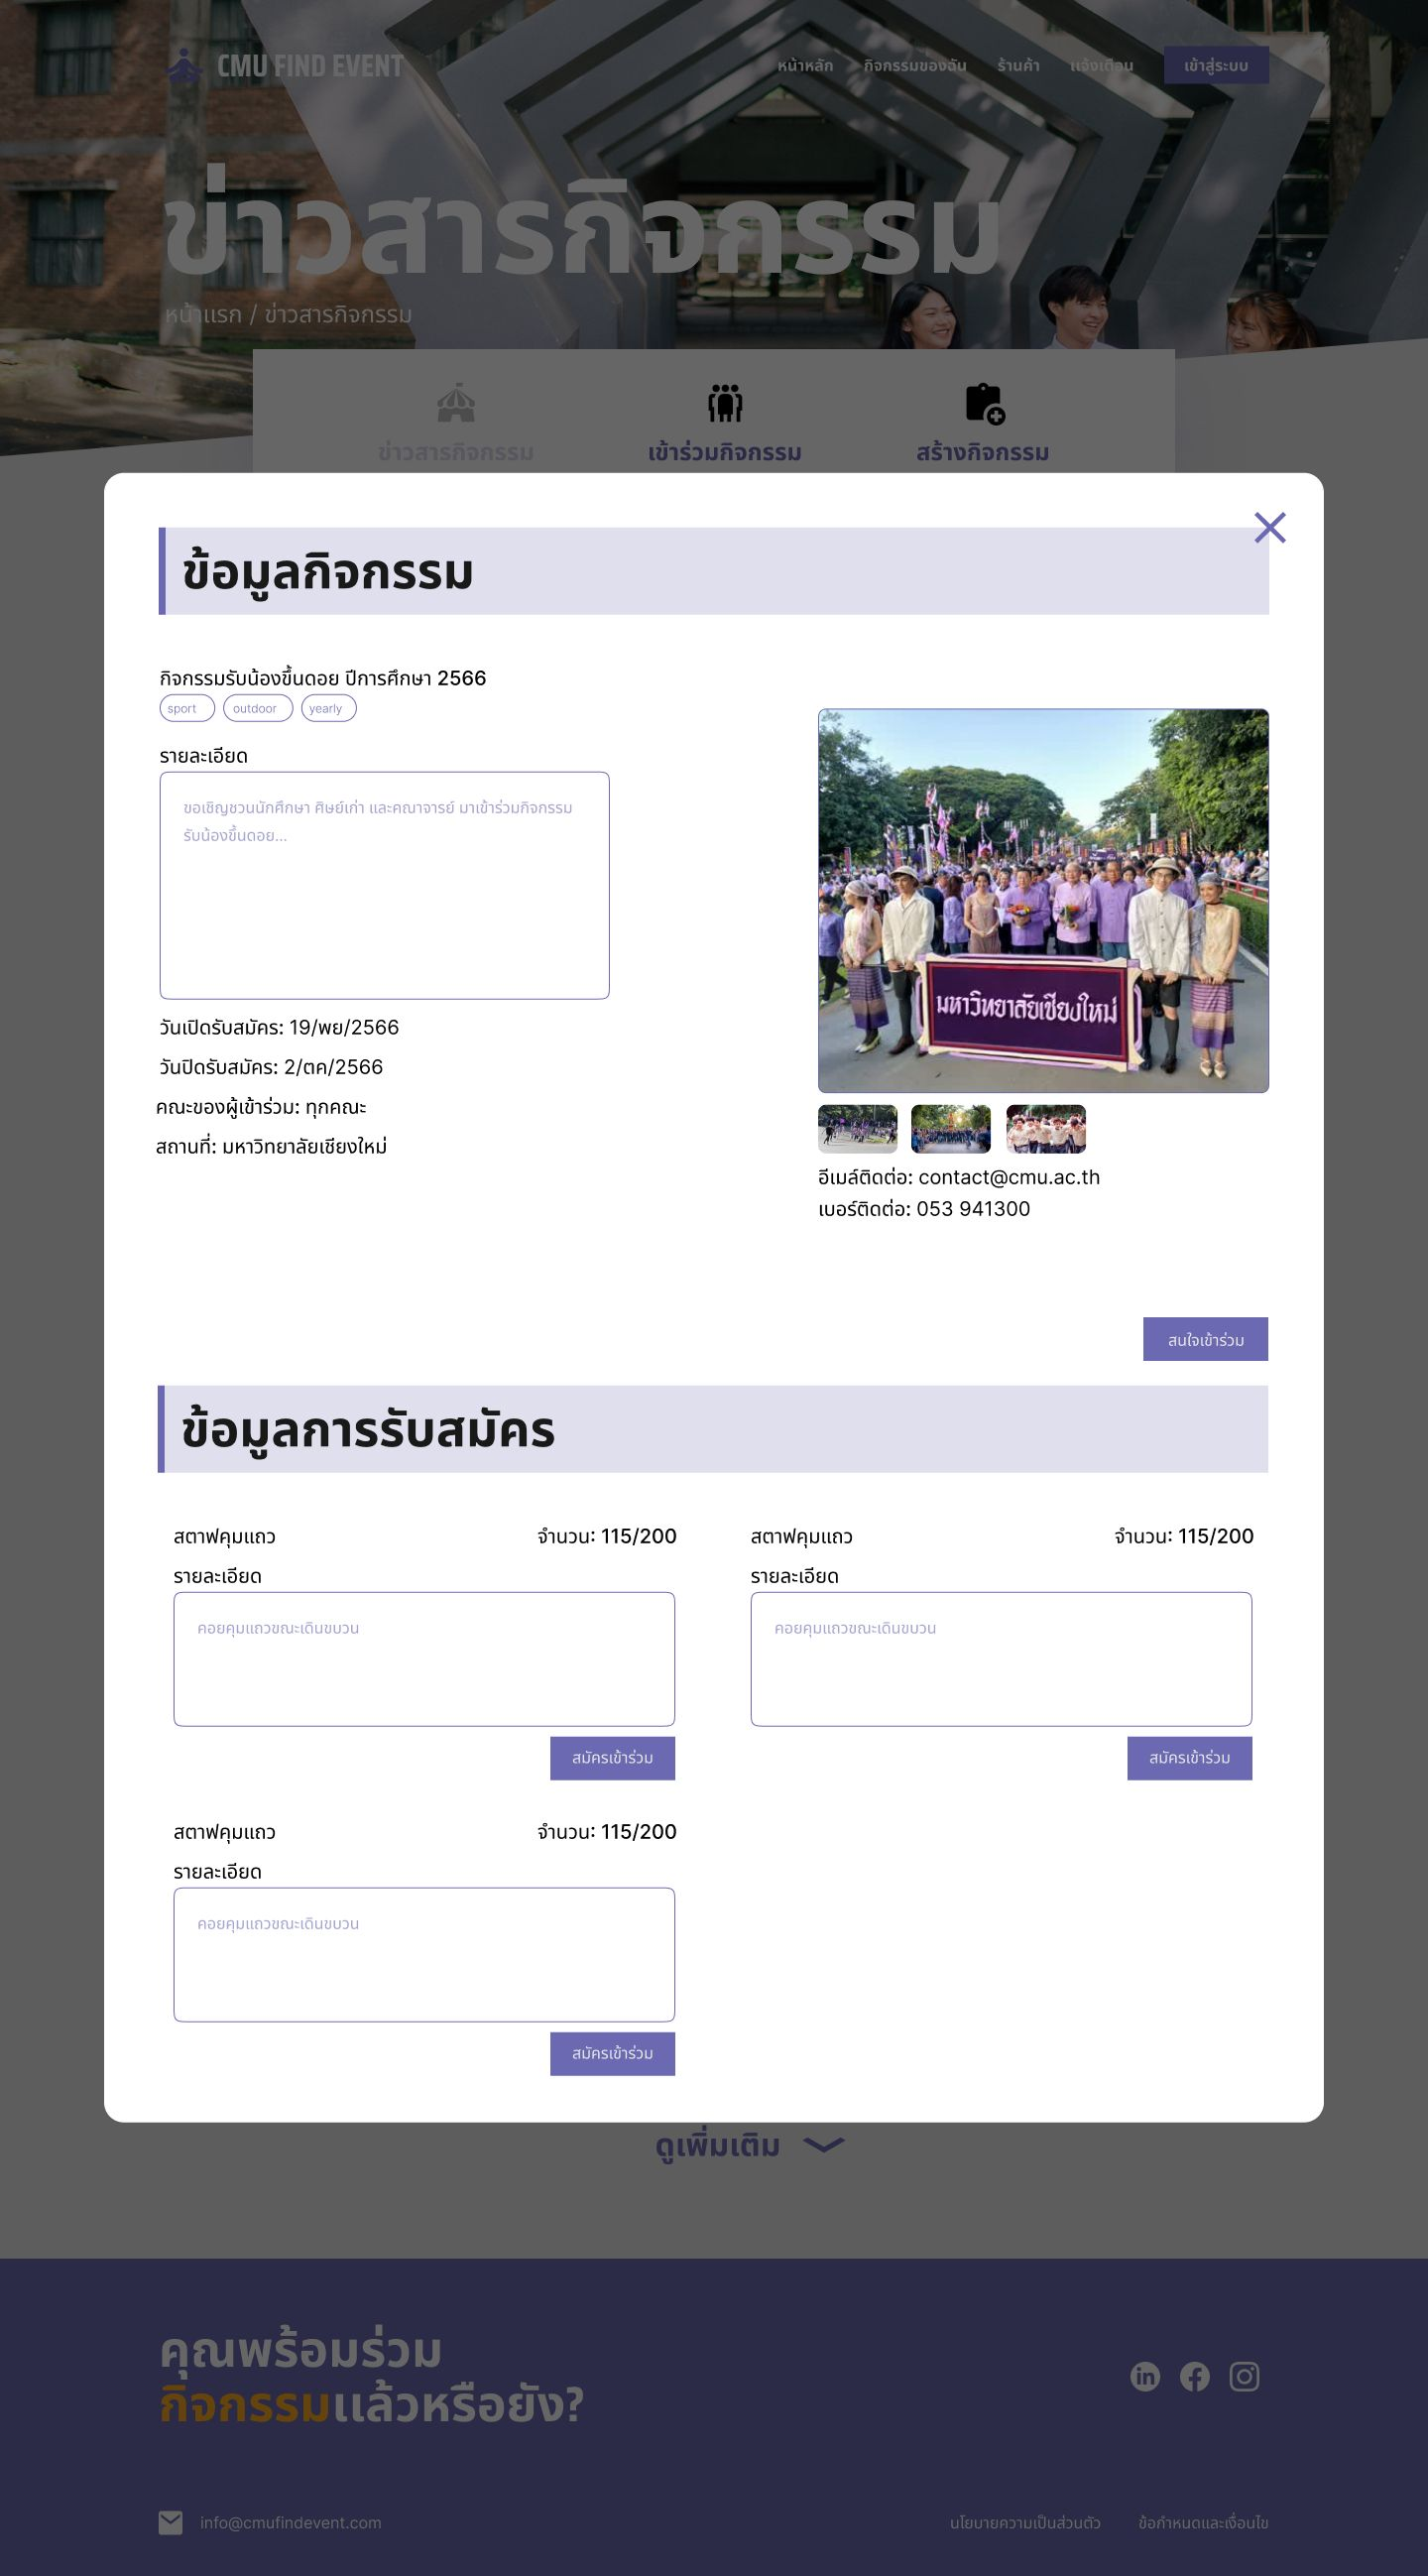
\includegraphics[width=\linewidth]{image/Figma-design/New-Event-info2.jpg}
    \caption{แสดงรายละเอียดของกิจกรรม}
  \end{subfigure}
  \caption{หน้ารายการกิจกรรม}
  \label{fig:event-info}
\end{figure}

\begin{figure}[h]
  \centering
  \begin{subfigure}[b]{0.3\linewidth}
    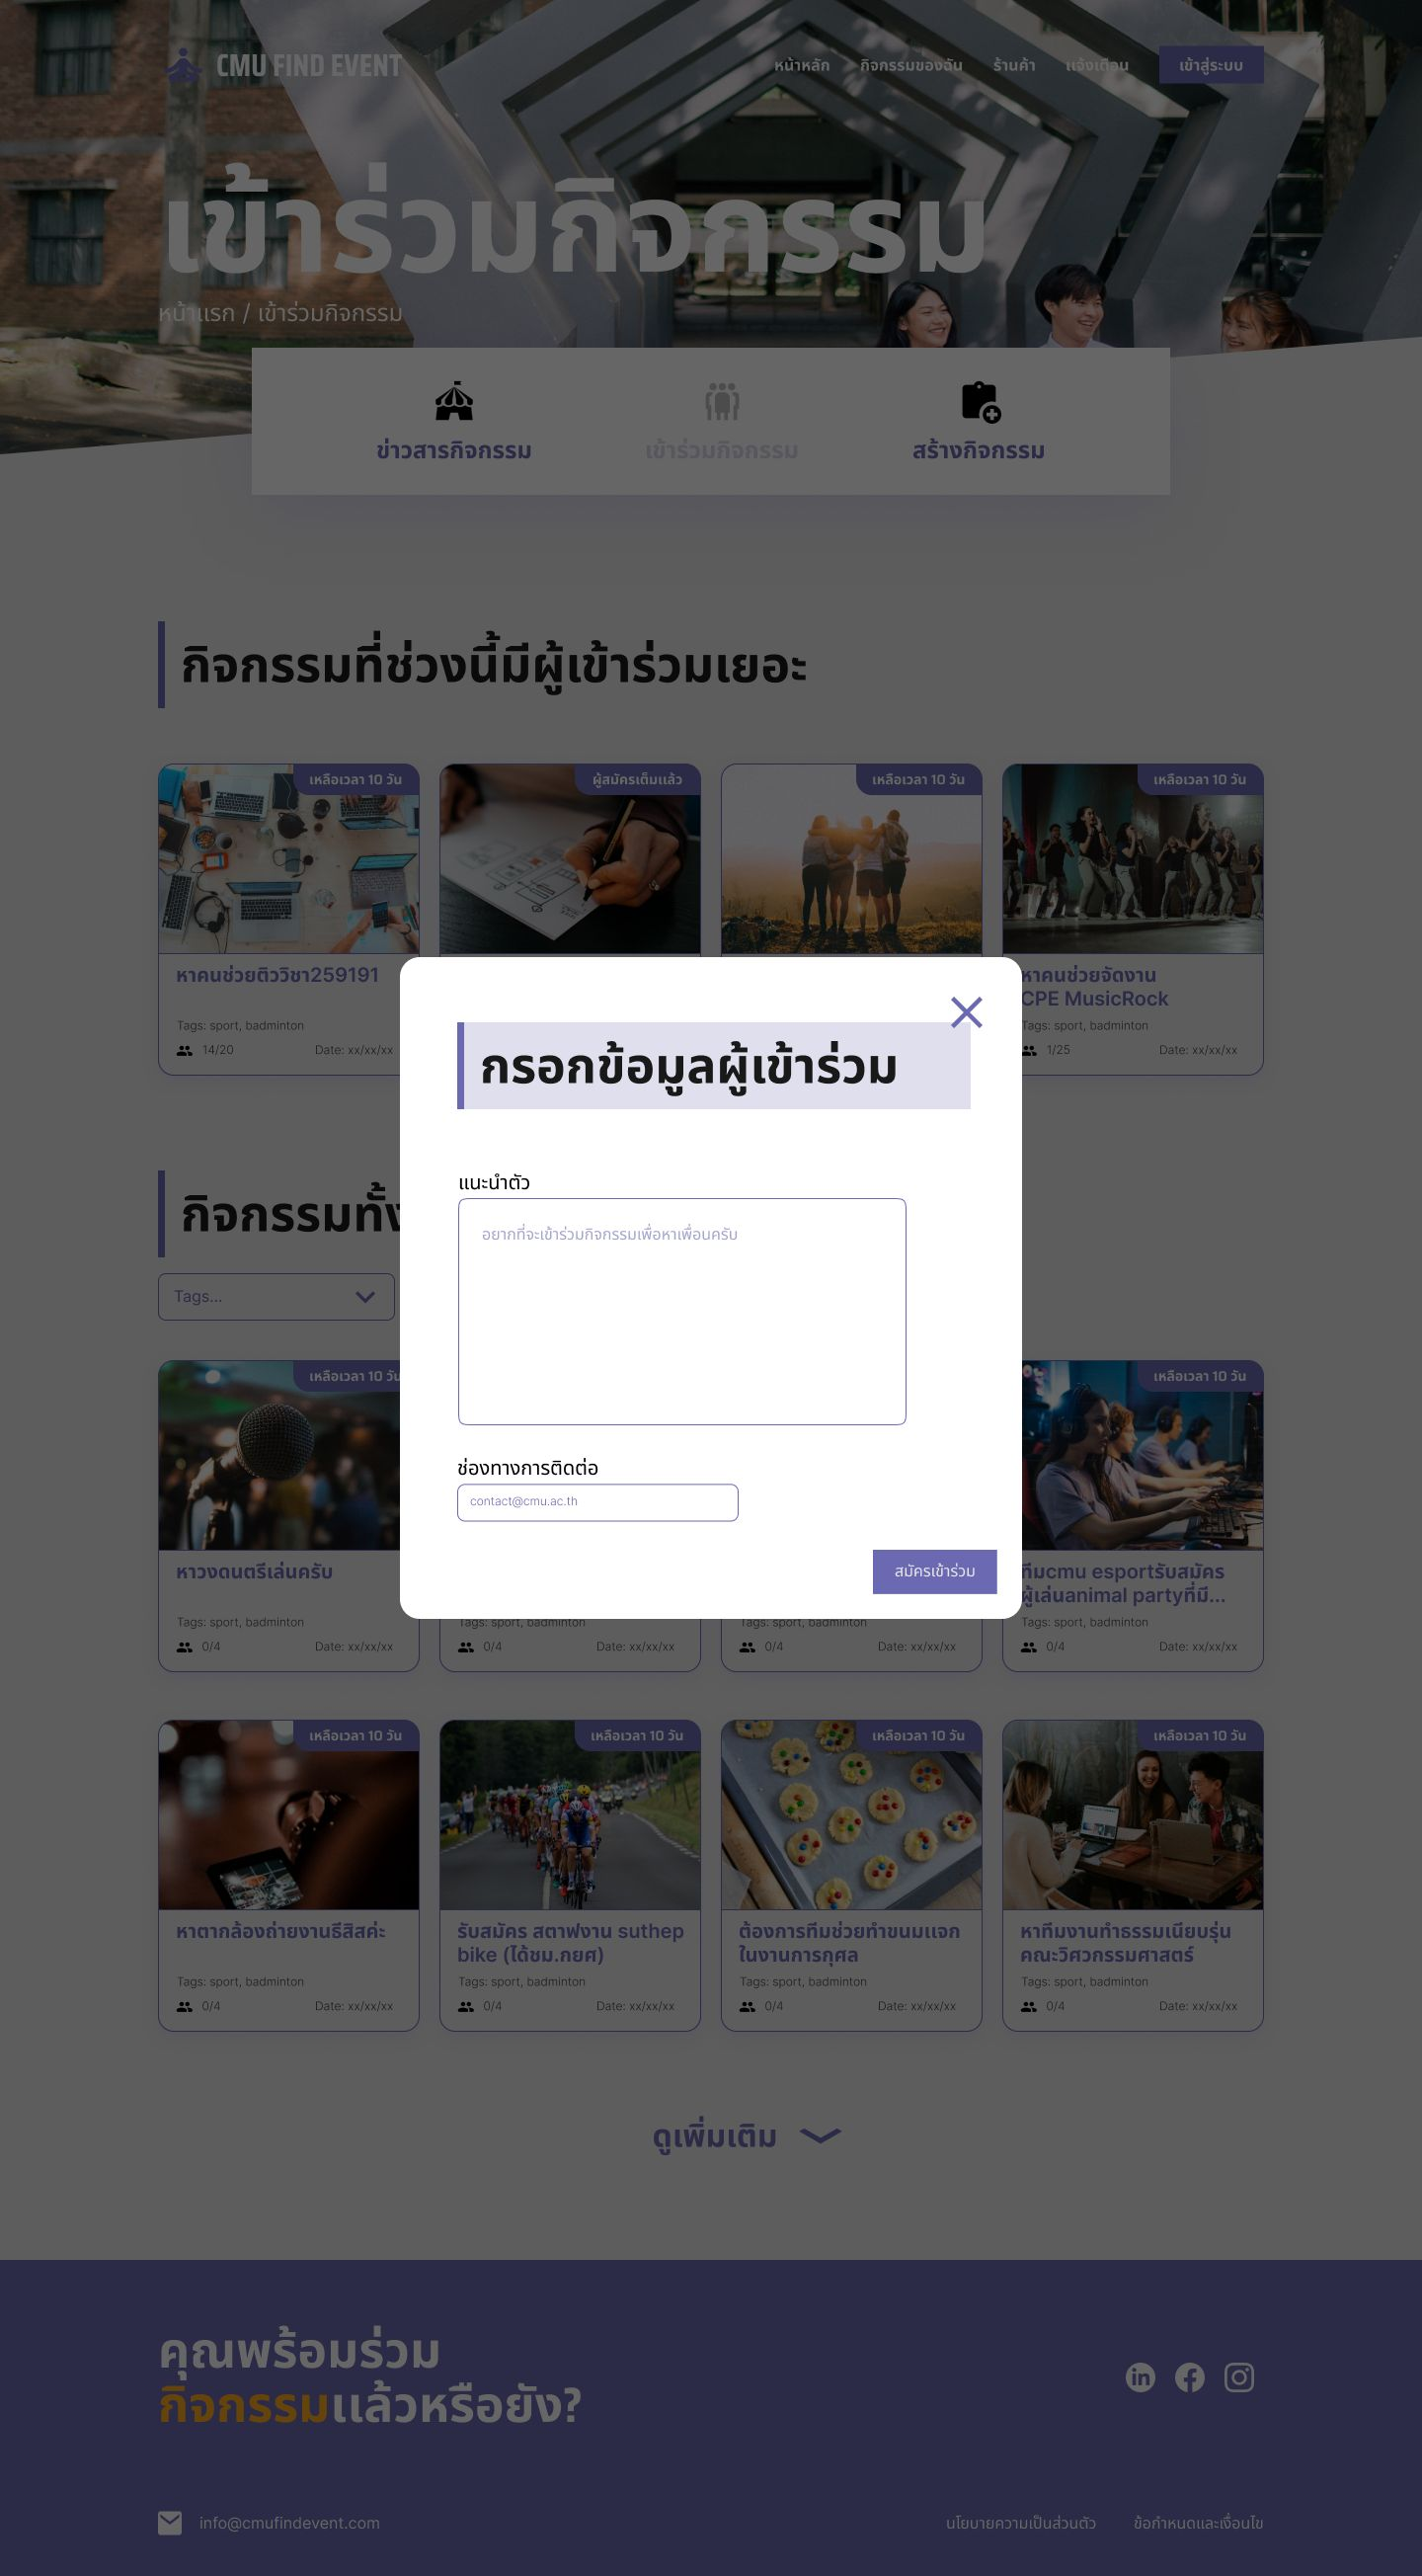
\includegraphics[width=\linewidth]{image/Figma-design/New-Event-join.jpg}
    \caption{แสดงหน้าคำขอเข้าร่วม}
  \end{subfigure}
  \hfill
  \begin{subfigure}[b]{0.3\linewidth}
    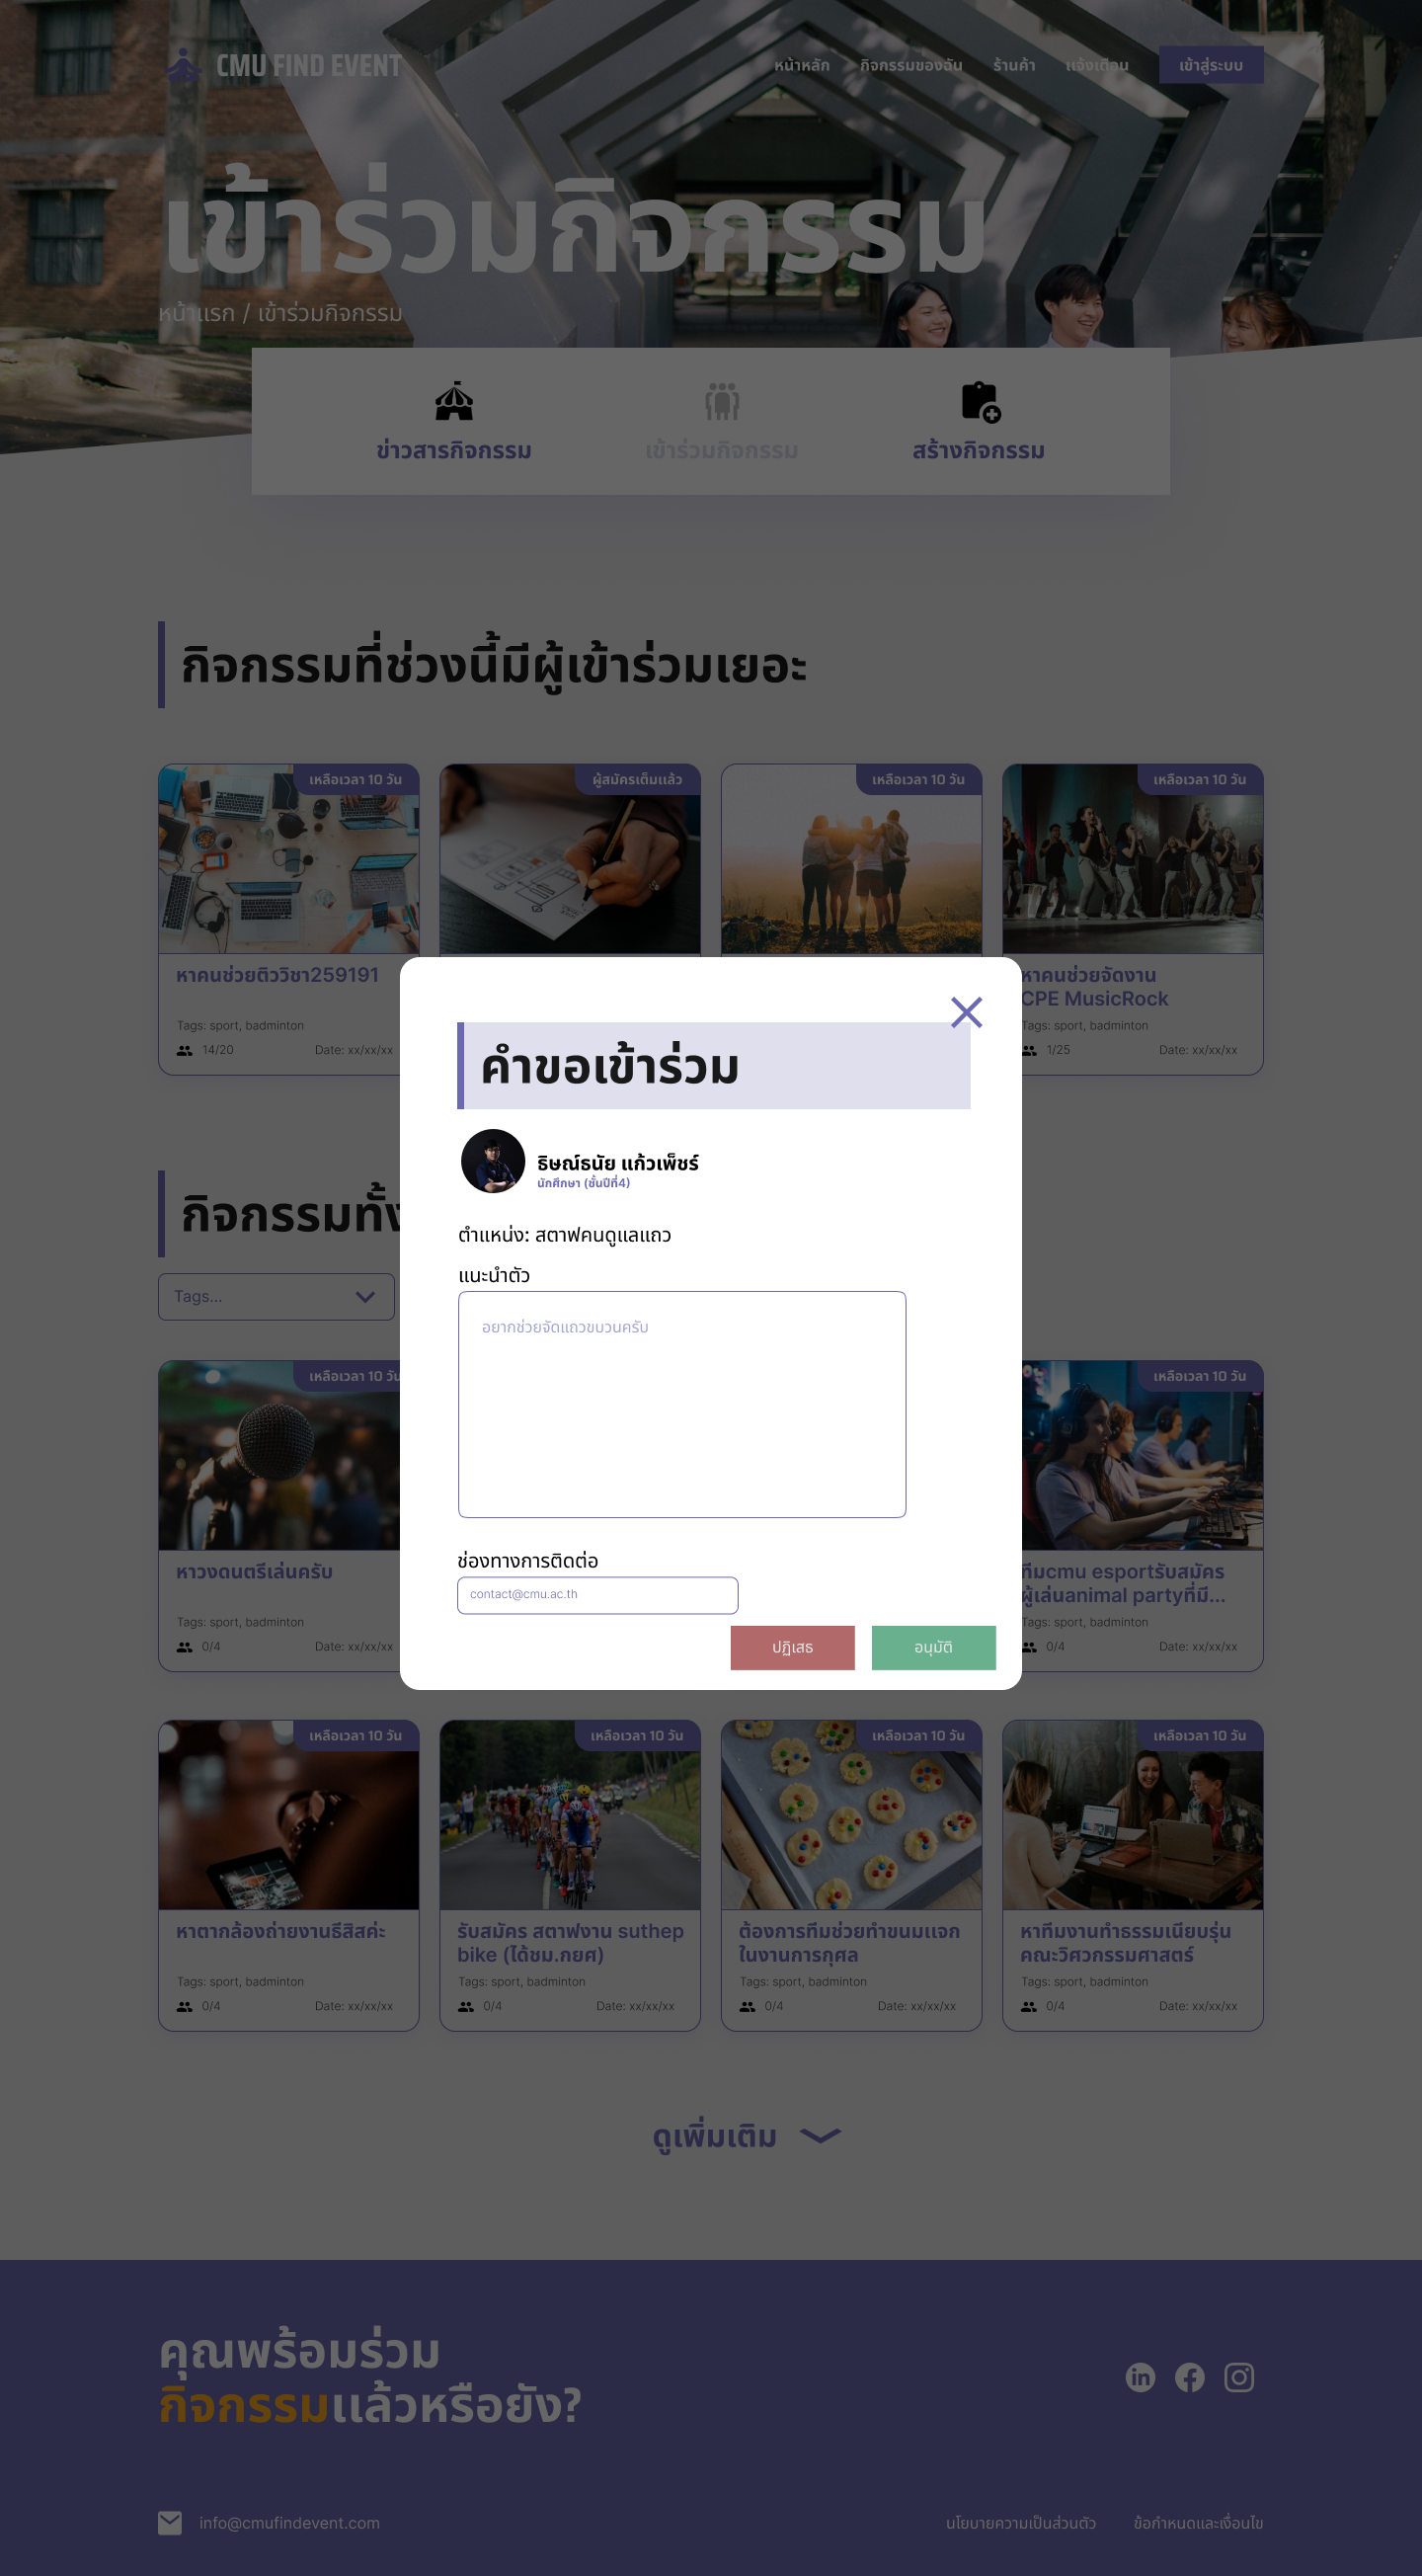
\includegraphics[width=\linewidth]{image/Figma-design/New-Event-join-noti.png}
    \caption{แสดงรายการคำขอเข้าร่วม}
  \end{subfigure}
  \caption{หน้าการขอเข้าร่วมกิจกรรม}
  \label{fig:event-join}
\end{figure}

\begin{figure}[h]
  \centering
  \begin{subfigure}[b]{0.3\linewidth}
    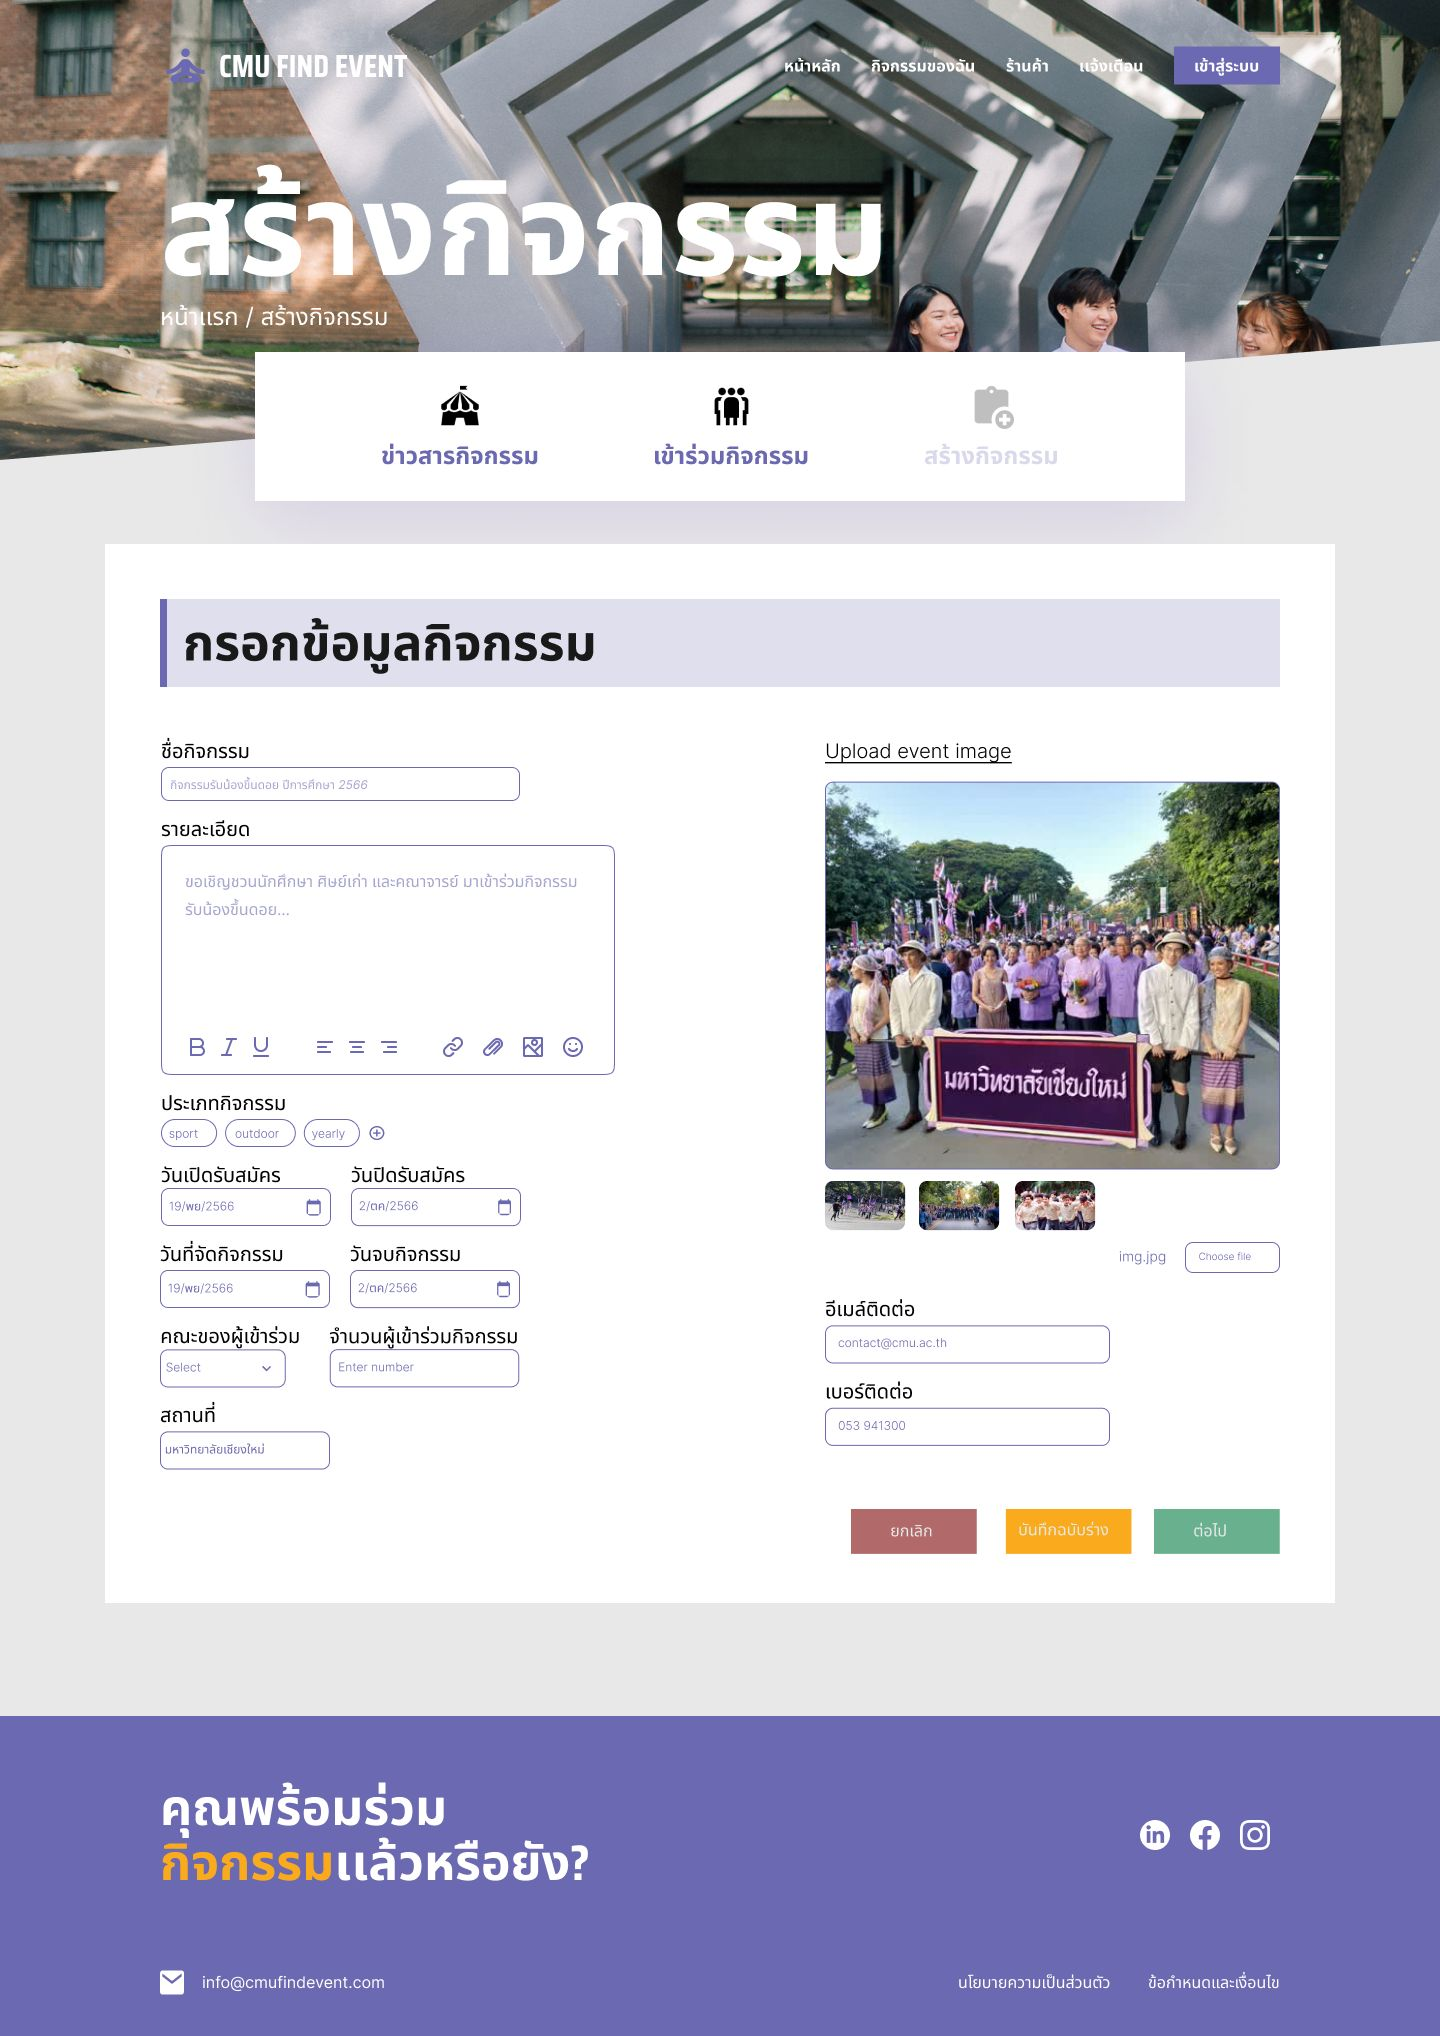
\includegraphics[width=\linewidth]{image/Figma-design/Create-event-info.jpg}
    \caption{กรอกข้อมูลสร้างกิจกรรม}
  \end{subfigure}
  \hfill
  \begin{subfigure}[b]{0.3\linewidth}
    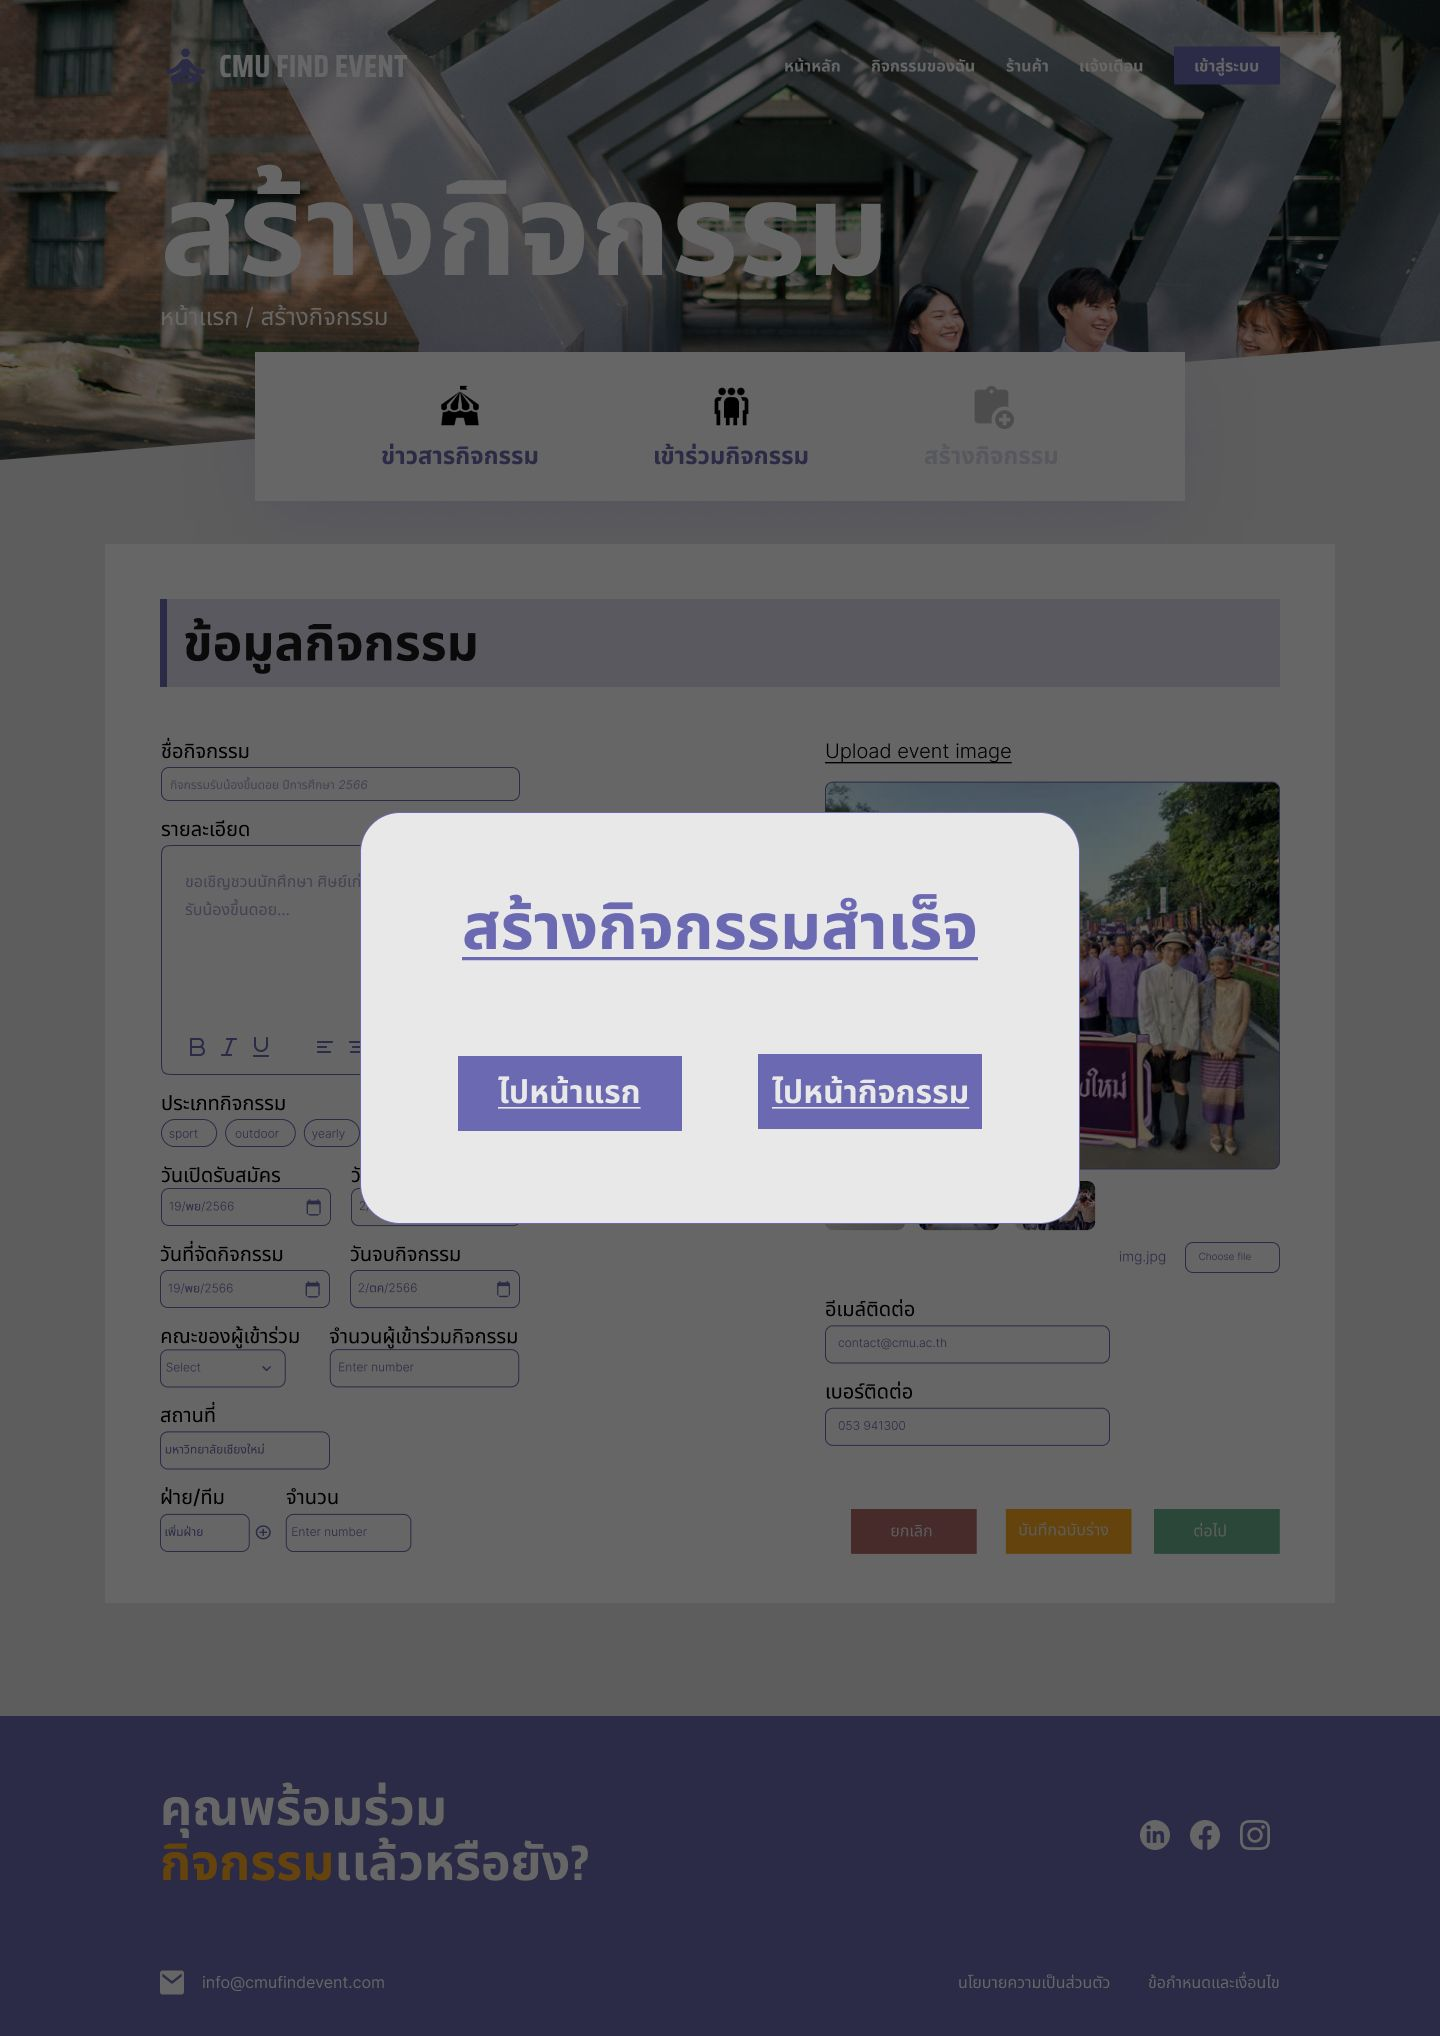
\includegraphics[width=\linewidth]{image/Figma-design/Create-event-info-1.jpg}
    \caption{แสดงข้อความสร้างสำเร็จ}
  \end{subfigure}
  \caption{หน้าสร้างกิจกรรม}
  \label{fig:event-create}
\end{figure}

\begin{figure}[h]
  \centering
  \begin{subfigure}[b]{0.3\linewidth}
    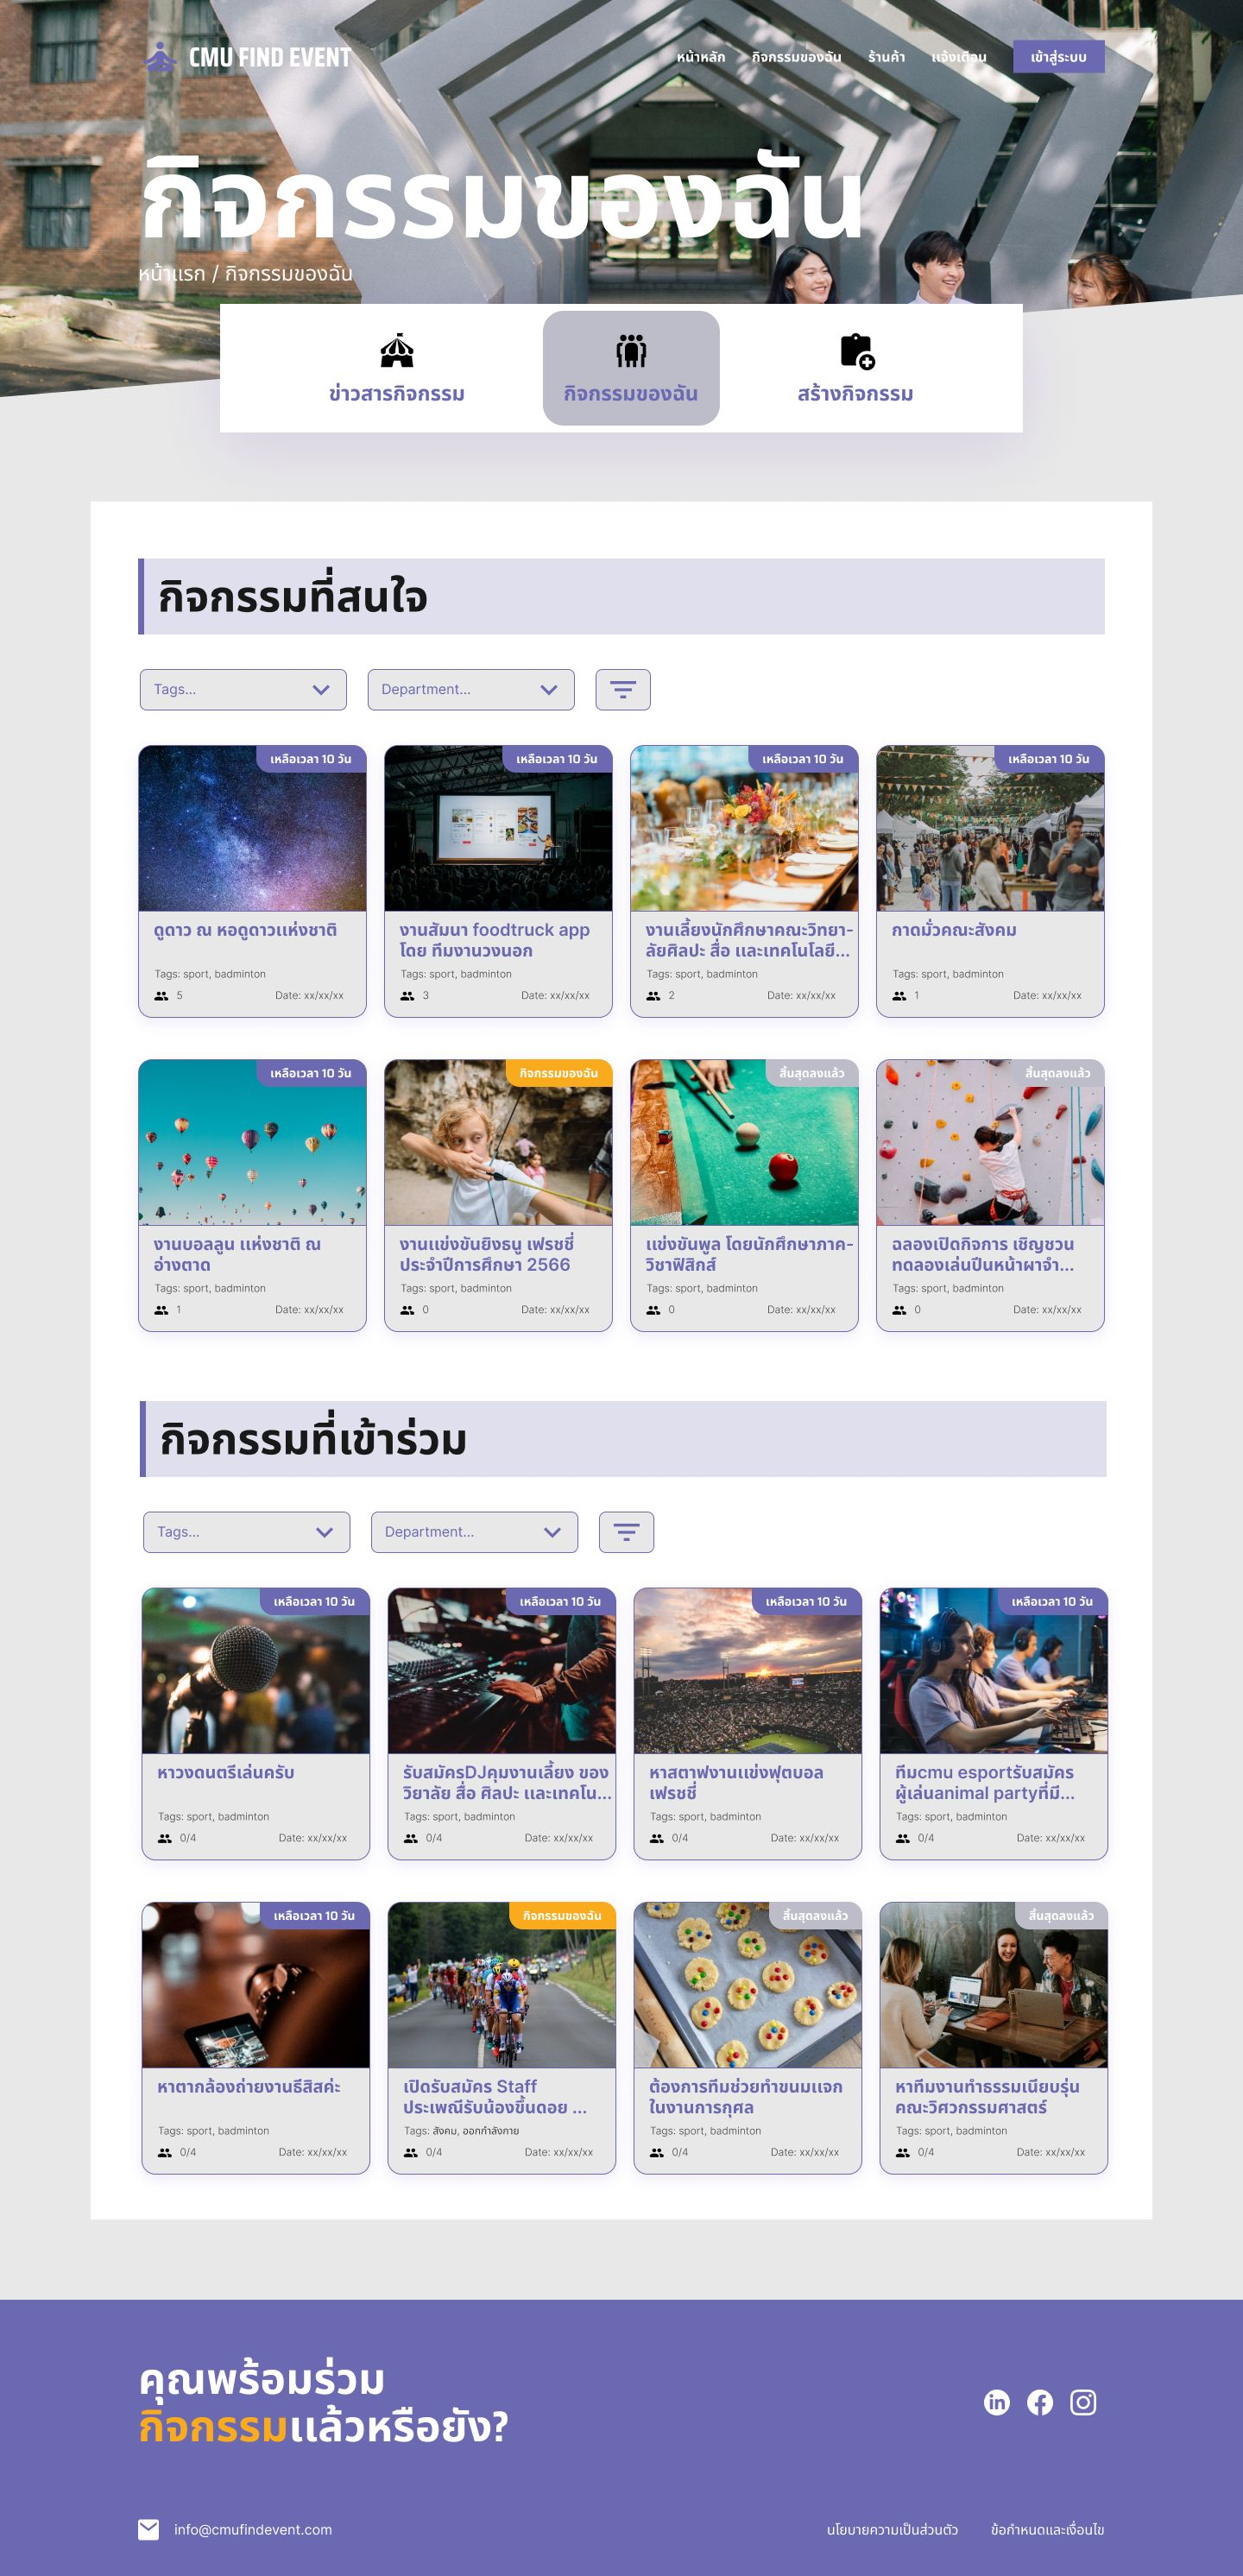
\includegraphics[width=\linewidth]{image/Figma-design/New-Mine-event.jpg}
    \caption{แสดงกิจกรรมที่เข้าร่วมอยู่}
  \end{subfigure}
  \hfill
  \begin{subfigure}[b]{0.3\linewidth}
    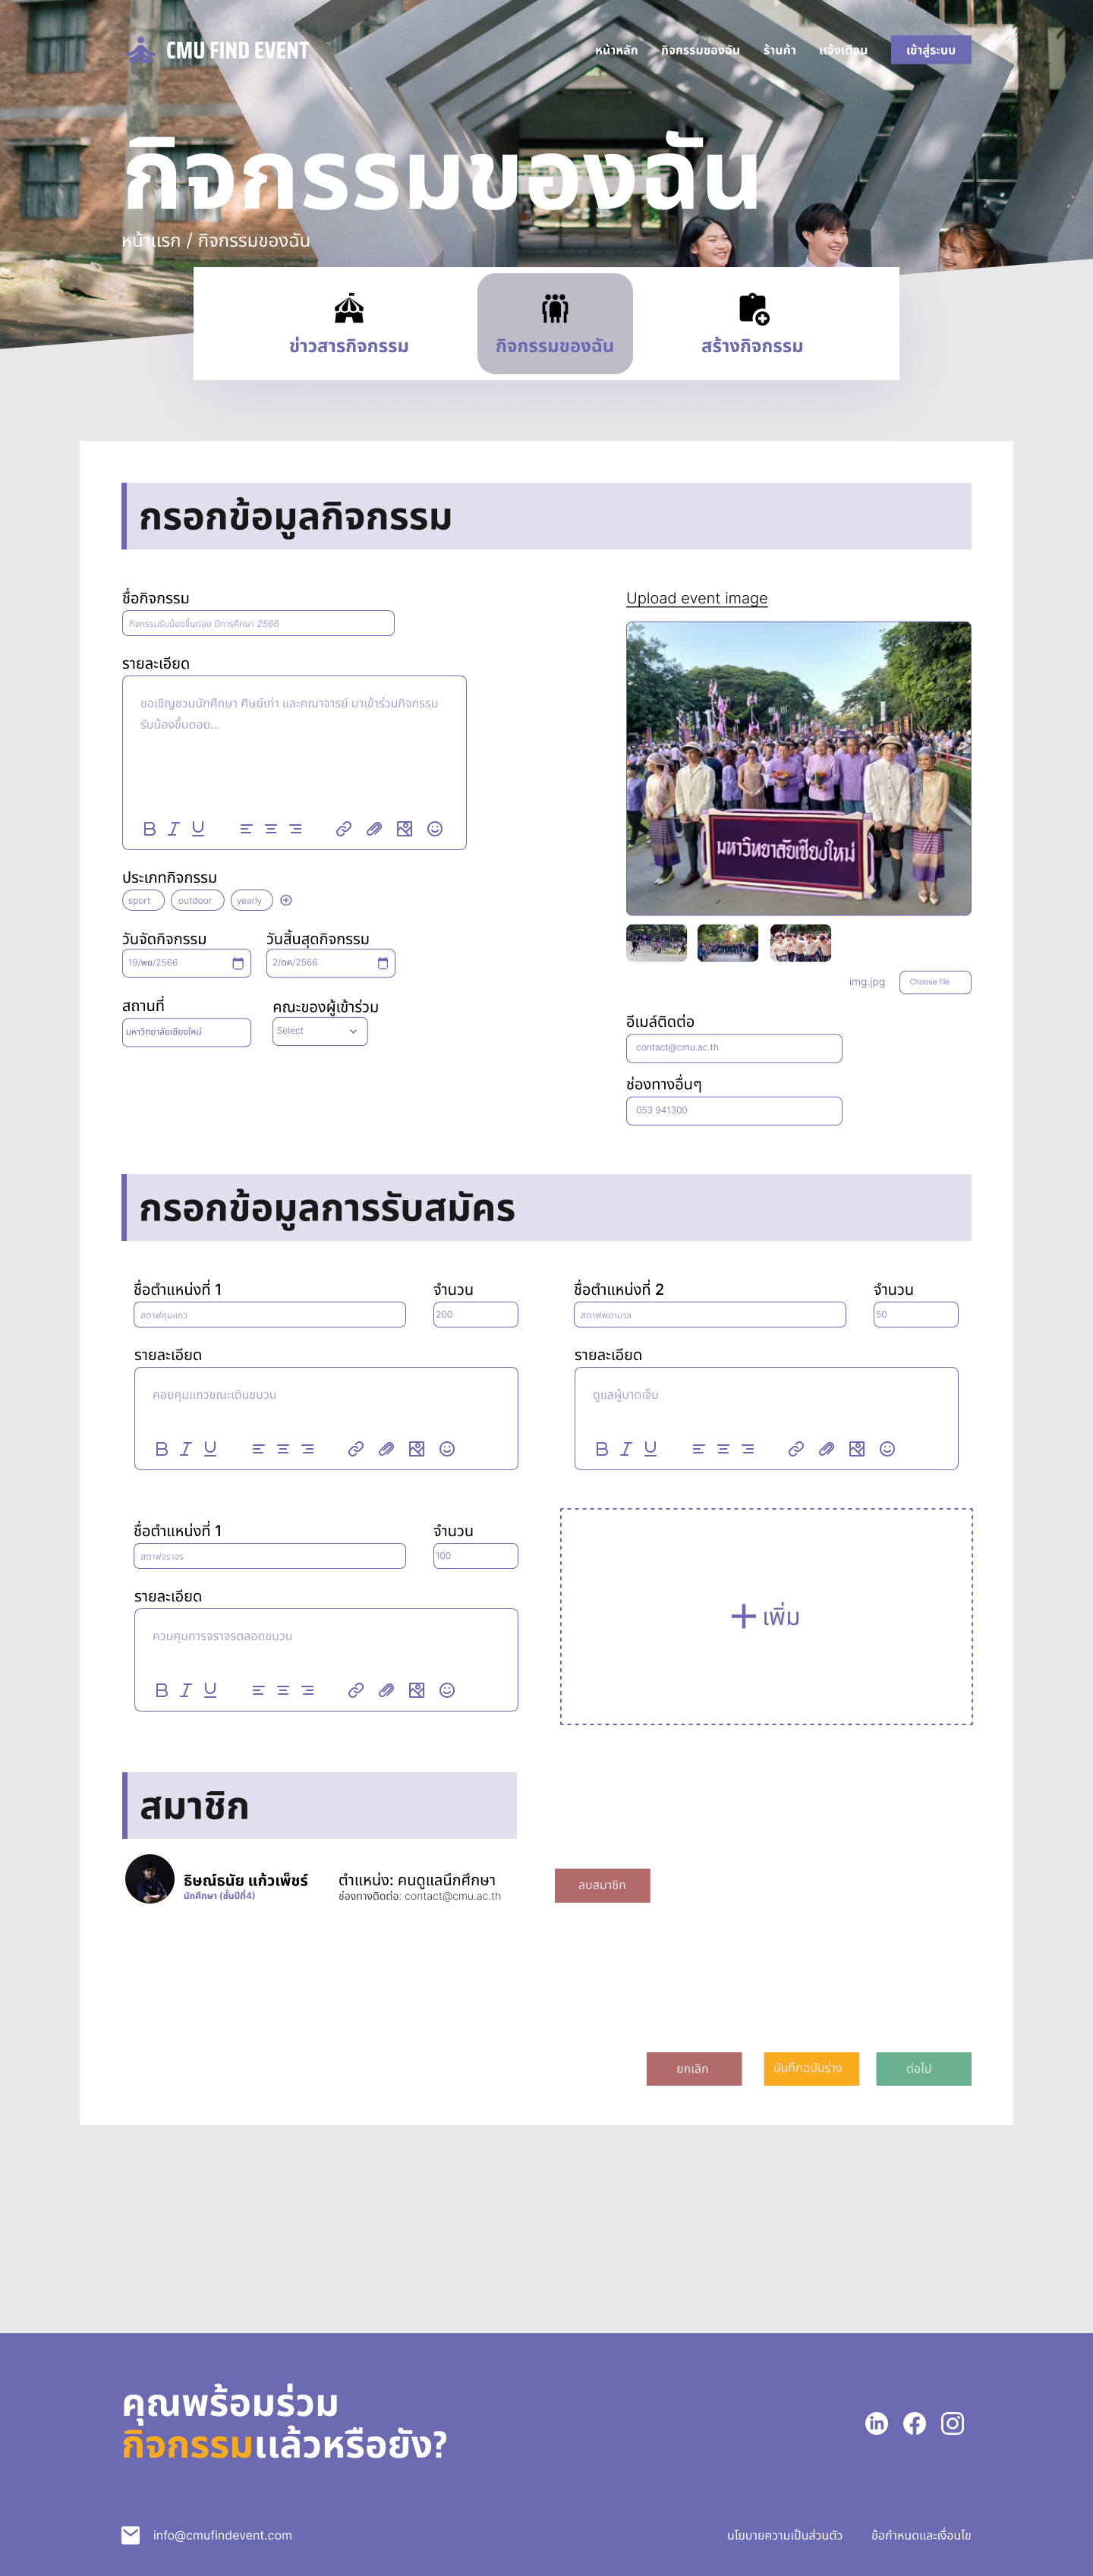
\includegraphics[width=\linewidth]{image/Figma-design/New-Mine-event2.png}
    \caption{แสดงรายละเอียดกิจกรรมที่เข้าร่วมอยู่}
  \end{subfigure}
  \caption{หน้ารายการกิจกรรมที่เข้าร่วม}
  \label{fig:event-mine}
\end{figure}

\begin{figure}[h]
  \centering
  \begin{subfigure}[b]{0.3\linewidth}
    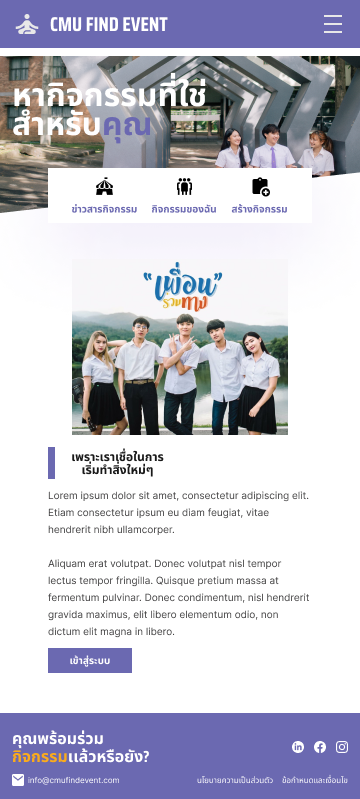
\includegraphics[width=\linewidth]{image/Figma-design/mobile-main.png}
    \caption{แสดงหน้าแรก}
  \end{subfigure}
  \hfill
  \begin{subfigure}[b]{0.3\linewidth}
    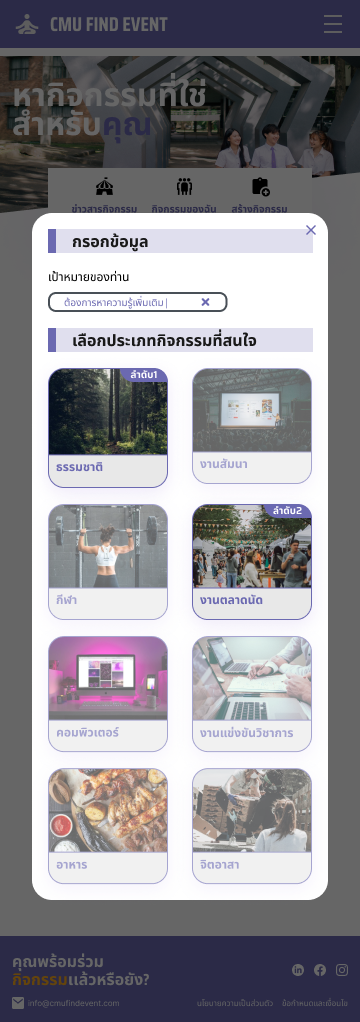
\includegraphics[width=\linewidth]{image/Figma-design/mobile-recomendation.png}
    \caption{แสดงแบบสอบถามความสนใจ}
  \end{subfigure}
  \caption{หน้าการแสดงผลในโทรศัพท์}
  \label{fig:mobile}
\end{figure}

\FloatBarrier

\section{โครงสร้างการไหลของข้อมูล}
โครงสร้างการไหลของข้อมูลแบ่งออกเป็น 2 ส่วน ได้แก่ ข้อมูลผู้ใช้ ที่อยู่ในฝั่งผู้สมัคร และฝั่งของผู้สร้างกิจกรรม
โดยข้อมูลที่ผู้สมัครจะส่งไปให้ ผู้สร้าง ได้แก่ ข้อมูลชื่อ นามสกุล และชั้นปีของผู้ใช้,ข้อมูลตำแหน่งที่ผู้ใช้สมัคร,ข้อความแนะนำตัว, ข้อมูลช่องทางติดต่อ 
ไปให้กับผู้สร้างกิจกรรม และผู้สร้างกิจกรรมสามารถตอบรับหรือปฎิเสธคำขอสมัครได้
\begin{figure}[h]
\begin{center}
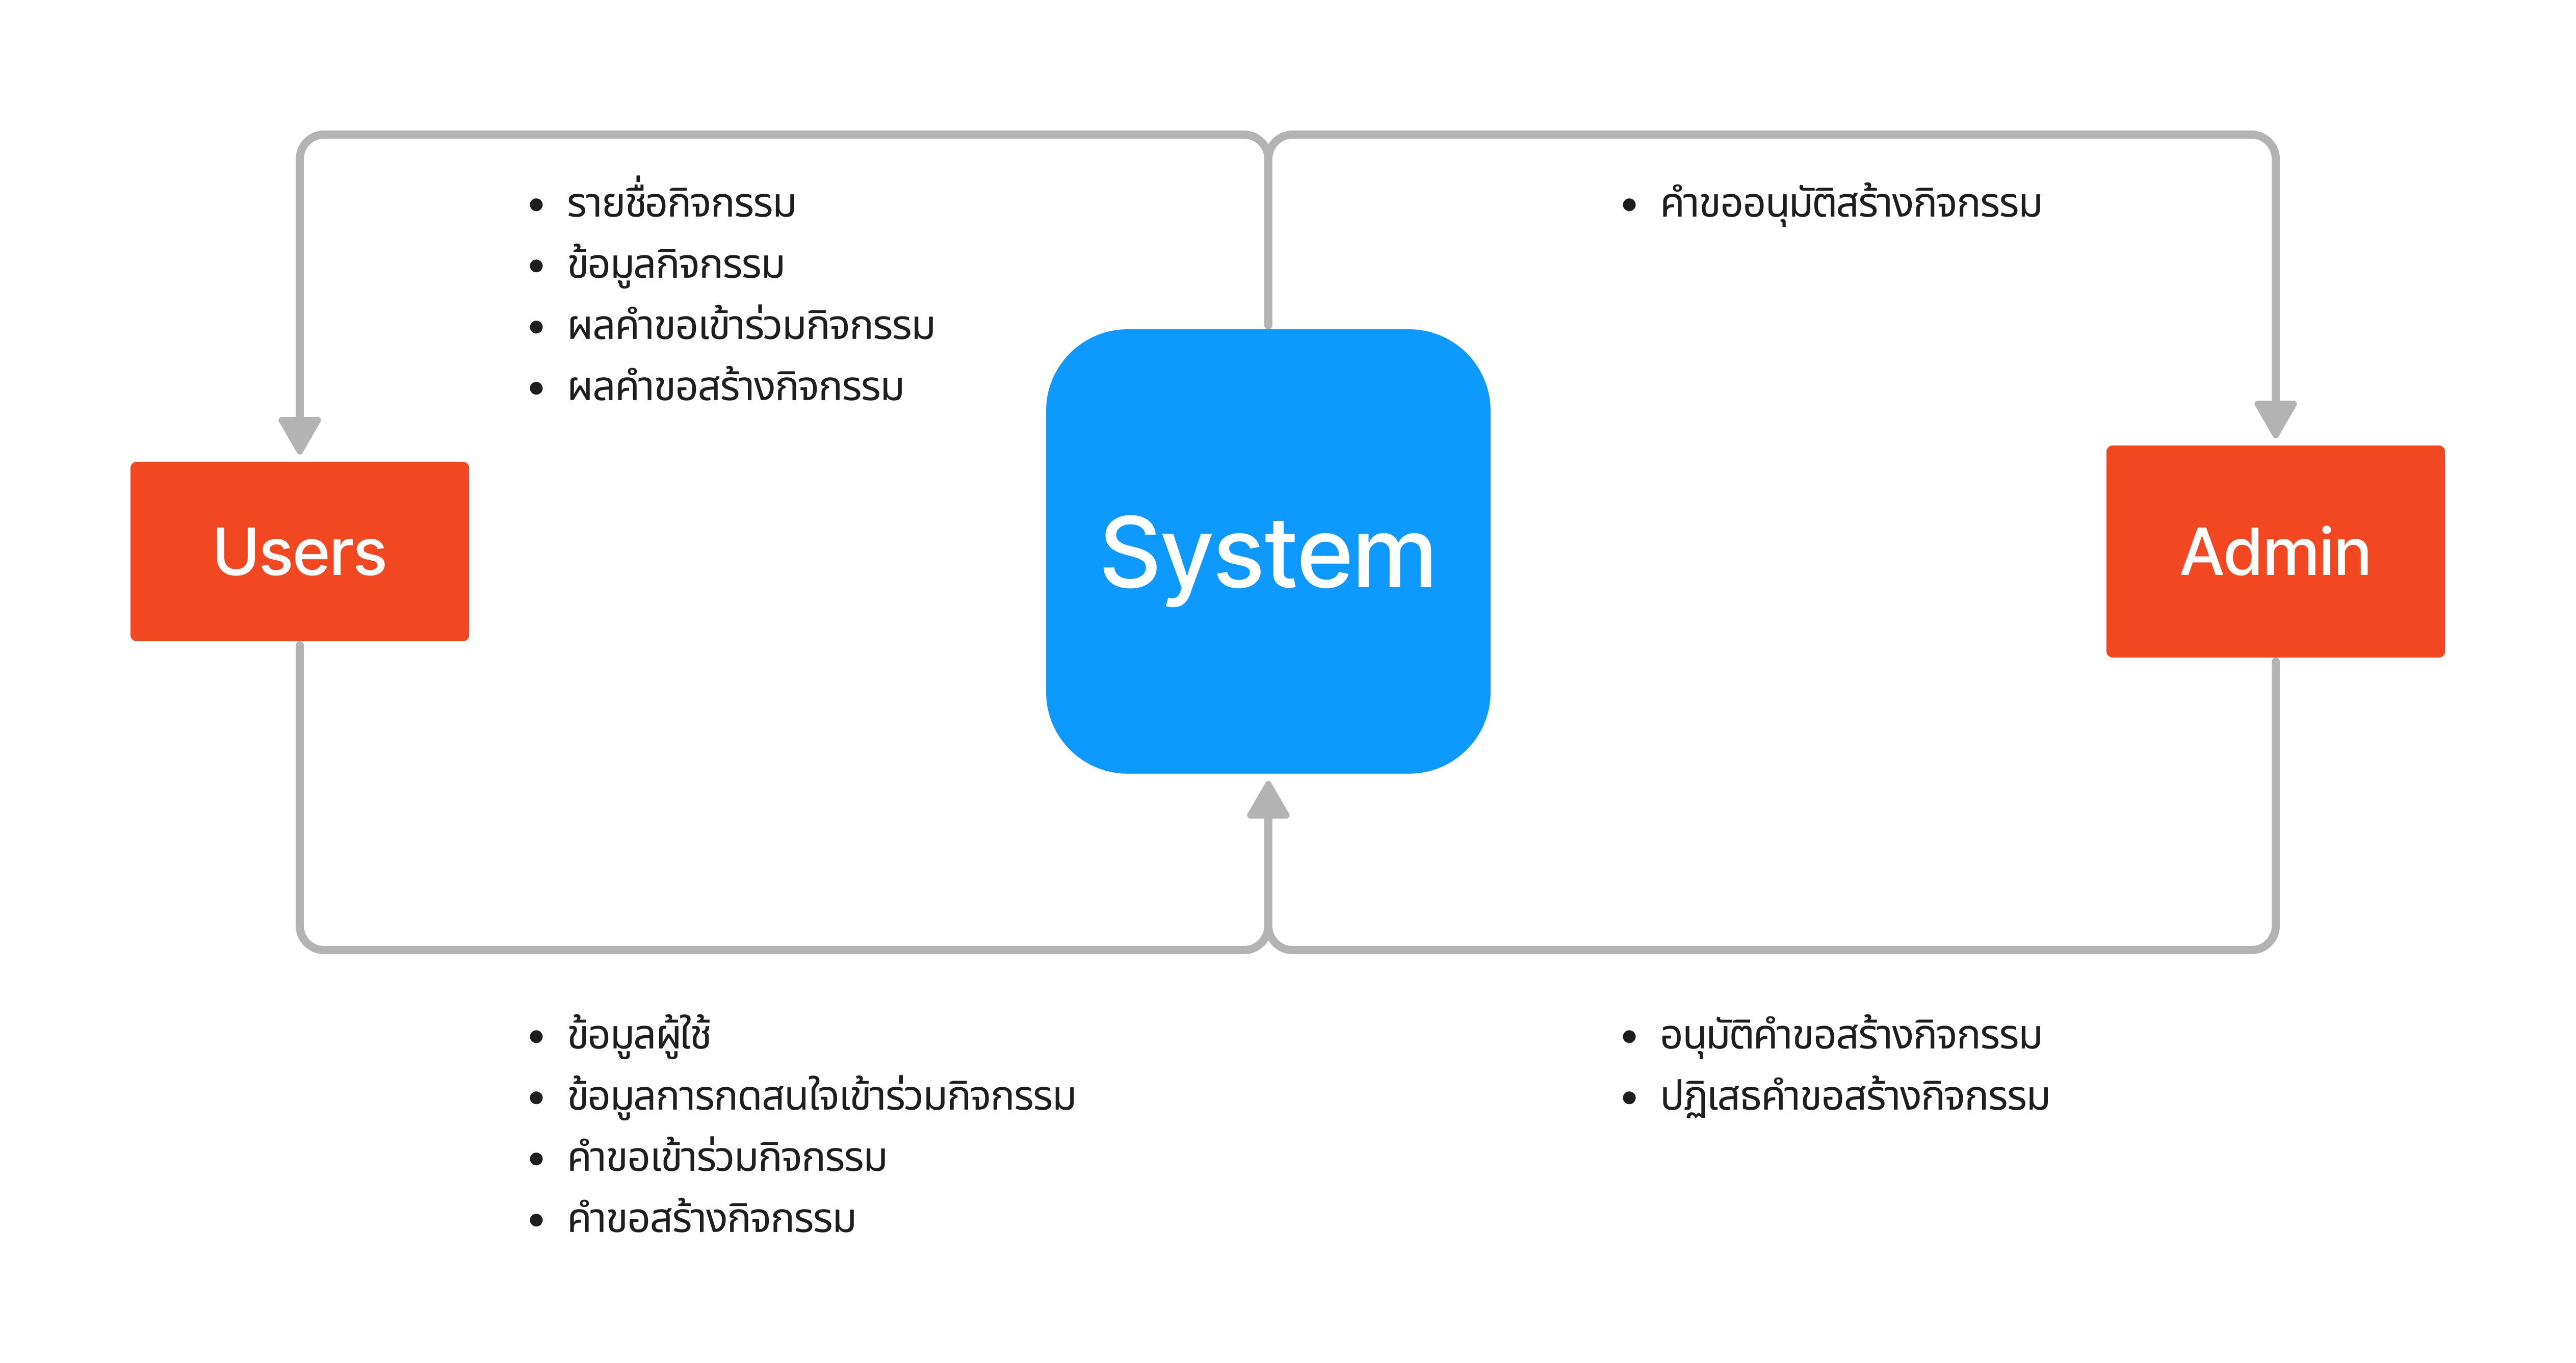
\includegraphics[width=0.9\linewidth]{image/dataflow-diagram.png}
\end{center}
\caption{แผนผังการไหลของข้อมูล}
\label{fig:dataflow}
\end{figure}
% \subsection{The Black Kitten}
%   One thing was certain, that the WHITE kitten had had nothing to
% do with it:---it was the black kitten's fault entirely~\cite{aiw}.  For the
% white kitten had been having its face washed by the old cat for
% the last quarter of an hour (and bearing it pretty well,
% considering); so you see that it COULDN'T have had any hand in
% the mischief.

%   The way Dinah washed her children's faces was this:  first she
% held the poor thing down by its ear with one paw, and then with
% the other paw she rubbed its face all over, the wrong way,
% beginning at the nose:  and just now, as I said, she was hard at
% work on the white kitten, which was lying quite still and trying
% to purr---no doubt feeling that it was all meant for its good.

%   But the black kitten had been finished with earlier in the
% afternoon, and so, while Alice was sitting curled up in a corner
% of the great arm-chair, half talking to herself and half asleep,
% the kitten had been having a grand game of romps with the ball of
% worsted Alice had been trying to wind up, and had been rolling it
% up and down till it had all come undone again; and there it was,
% spread over the hearth-rug, all knots and tangles, with the
% kitten running after its own tail in the middle.

% \subsection{The Reproach}

%   `Oh, you wicked little thing!' cried Alice, catching up the
% kitten, and giving it a little kiss to make it understand that it
% was in disgrace.  `Really, Dinah ought to have taught you better
% manners!  You OUGHT, Dinah, you know you ought!' she added,
% looking reproachfully at the old cat, and speaking in as cross a
% voice as she could manage---and then she scrambled back into the
% arm-chair, taking the kitten and the worsted with her, and began
% winding up the ball again.  But she didn't get on very fast, as
% she was talking all the time, sometimes to the kitten, and
% sometimes to herself.  Kitty sat very demurely on her knee,
% pretending to watch the progress of the winding, and now and then
% putting out one paw and gently touching the ball, as if it would
% be glad to help, if it might.

%   `Do you know what to-morrow is, Kitty?' Alice began.  `You'd
% have guessed if you'd been up in the window with me---only Dinah
% was making you tidy, so you couldn't.  I was watching the boys
% getting in stick for the bonfire---and it wants plenty of
% sticks, Kitty!  Only it got so cold, and it snowed so, they had
% to leave off.  Never mind, Kitty, we'll go and see the bonfire
% to-morrow.'  Here Alice wound two or three turns of the worsted
% round the kitten's neck, just to see how it would look:  this led
% to a scramble, in which the ball rolled down upon the floor, and
% yards and yards of it got unwound again.

%   `Do you know, I was so angry, Kitty,' Alice went on as soon as
% they were comfortably settled again, `when I saw all the mischief
% you had been doing, I was very nearly opening the window, and
% putting you out into the snow!  And you'd have deserved it, you
% little mischievous darling!  What have you got to say for
% yourself?  Now don't interrupt me!' she went on, holding up one
% finger.  `I'm going to tell you all your faults.  Number one:
% you squeaked twice while Dinah was washing your face this
% morning.  Now you can't deny it, Kitty:  I heard you!  What that
% you say?' (pretending that the kitten was speaking.)  `Her paw
% went into your eye?  Well, that's YOUR fault, for keeping your
% eyes open---if you'd shut them tight up, it wouldn't have
% happened.  Now don't make any more excuses, but listen!  Number
% two:  you pulled Snowdrop away by the tail just as I had put down
% the saucer of milk before her!  What, you were thirsty, were you?
